
% Mathieu Kessler 
% Departamento de Matemática Aplicada y Estadística
% Universidad Politécnica de Cartagena

\documentclass[9pt]{beamer}
\definecolor{links}{HTML}{2A1B81}
\hypersetup{colorlinks,linkcolor=,urlcolor=links}
 \usepackage[spanish]{babel}
\usepackage{colortbl}
\usepackage{graphicx}
\usepackage{amsmath,amssymb}
\usepackage{comma}
\usepackage{fancybox,color}
\usepackage[utf8]{inputenc}
\graphicspath{{fig/}}
\setbeamertemplate{navigation symbols}{}
%\usepackage[colorlinks=true]{hyperref}


\usepackage{beamerthemeshadow}
\usepackage{xmpmulti}
% \usepackage{mathtools}
% \DeclarePairedDelimiter\abs{\lvert}{\rvert}%


\newcommand{\field}[1]{\mathbb{#1}}
\newcommand{\E}{\field{E}}
\newcommand{\R}{\field{R}}
\newcommand{\N}{\field{N}}
\newcommand{\Z}{\field{Z}}
\newcommand{\Q}{\field{Q}}
\newcommand{\EE}{\field{E}}
\newcommand{\FF}{\field{F}}
\newcommand{\GG}{\field{G}}
\renewcommand{\L}{\field{L}}
\renewcommand{\P}{\field{P}}
\newcommand{\LL}{{\mathfrak L}}

\begin{document}
\title{¿Están los p-valores condenados al destierro?}

\author[Mathieu Kessler]{Mathieu Kessler}
\institute[]{Universidad Politécnica de Cartagena}
\date{\textcolor{blue}{Almería, 25 de Noviembre de 2022}}
\titlegraphic{
\includegraphics[width=5cm]{images/adam_eva_Chagall}}

\begin{frame}
  \titlepage
\end{frame}
\begin{frame}
  \frametitle{¿Por qué estoy aquí?}
  \begin{overlayarea}{\textwidth}{\textheight}
    En febrero 2015:
    \begin{center}
      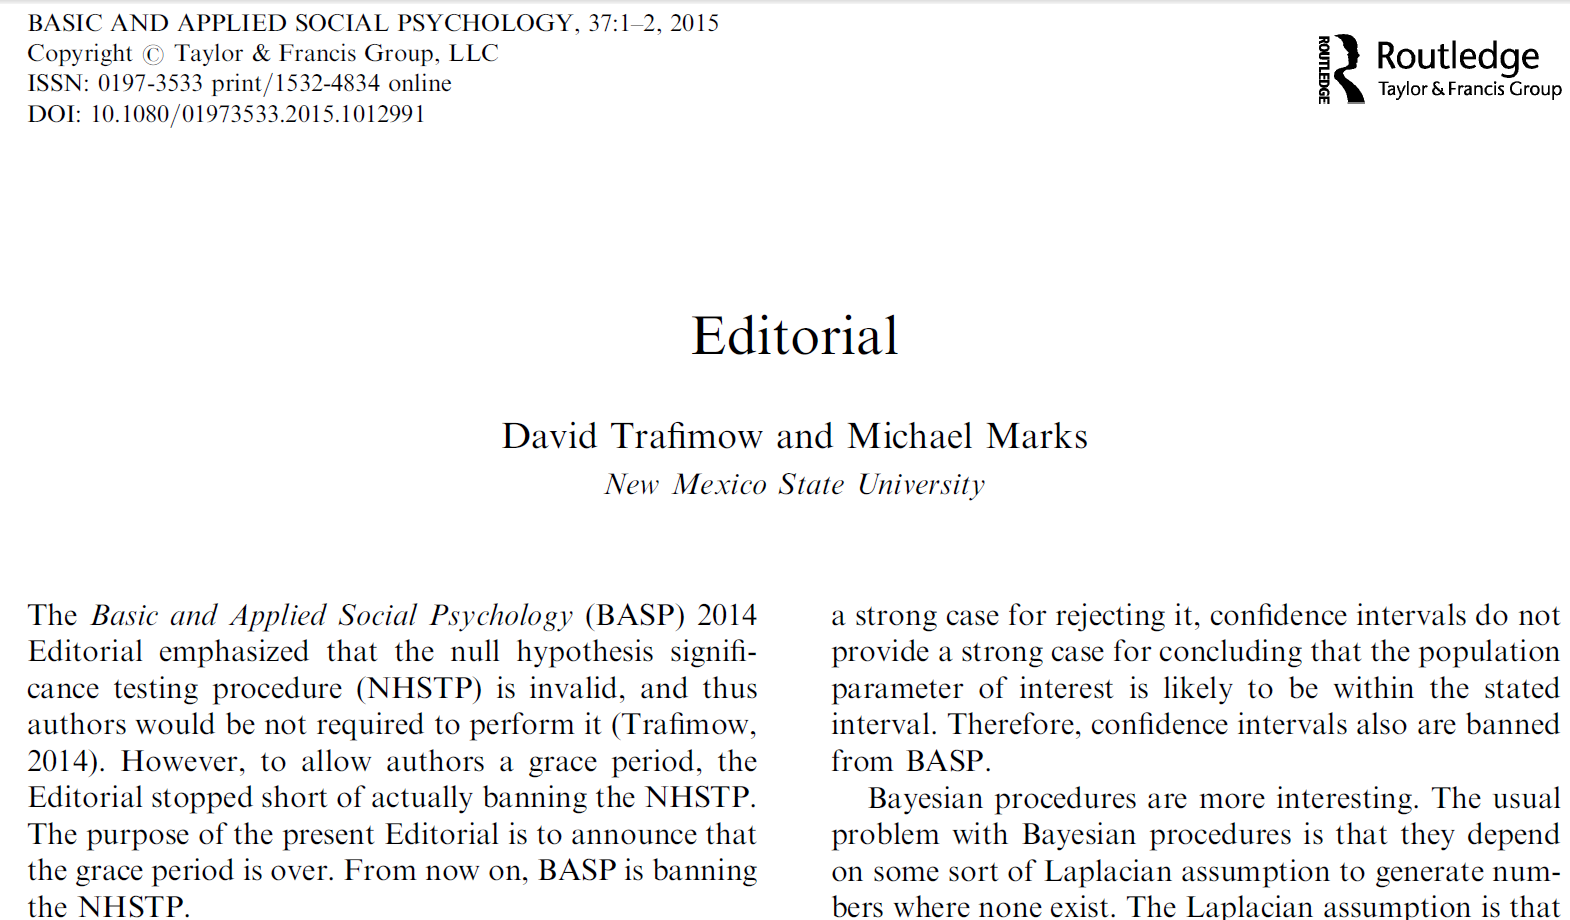
\includegraphics[width=8cm]{images/ban_editorial_0.png}
    \end{center}

  \end{overlayarea}
\end{frame}
\begin{frame}
  \frametitle{¿Por qué estoy aquí?}
  \begin{overlayarea}{\textwidth}{\textheight}
    En febrero 2015:
    \begin{center}
      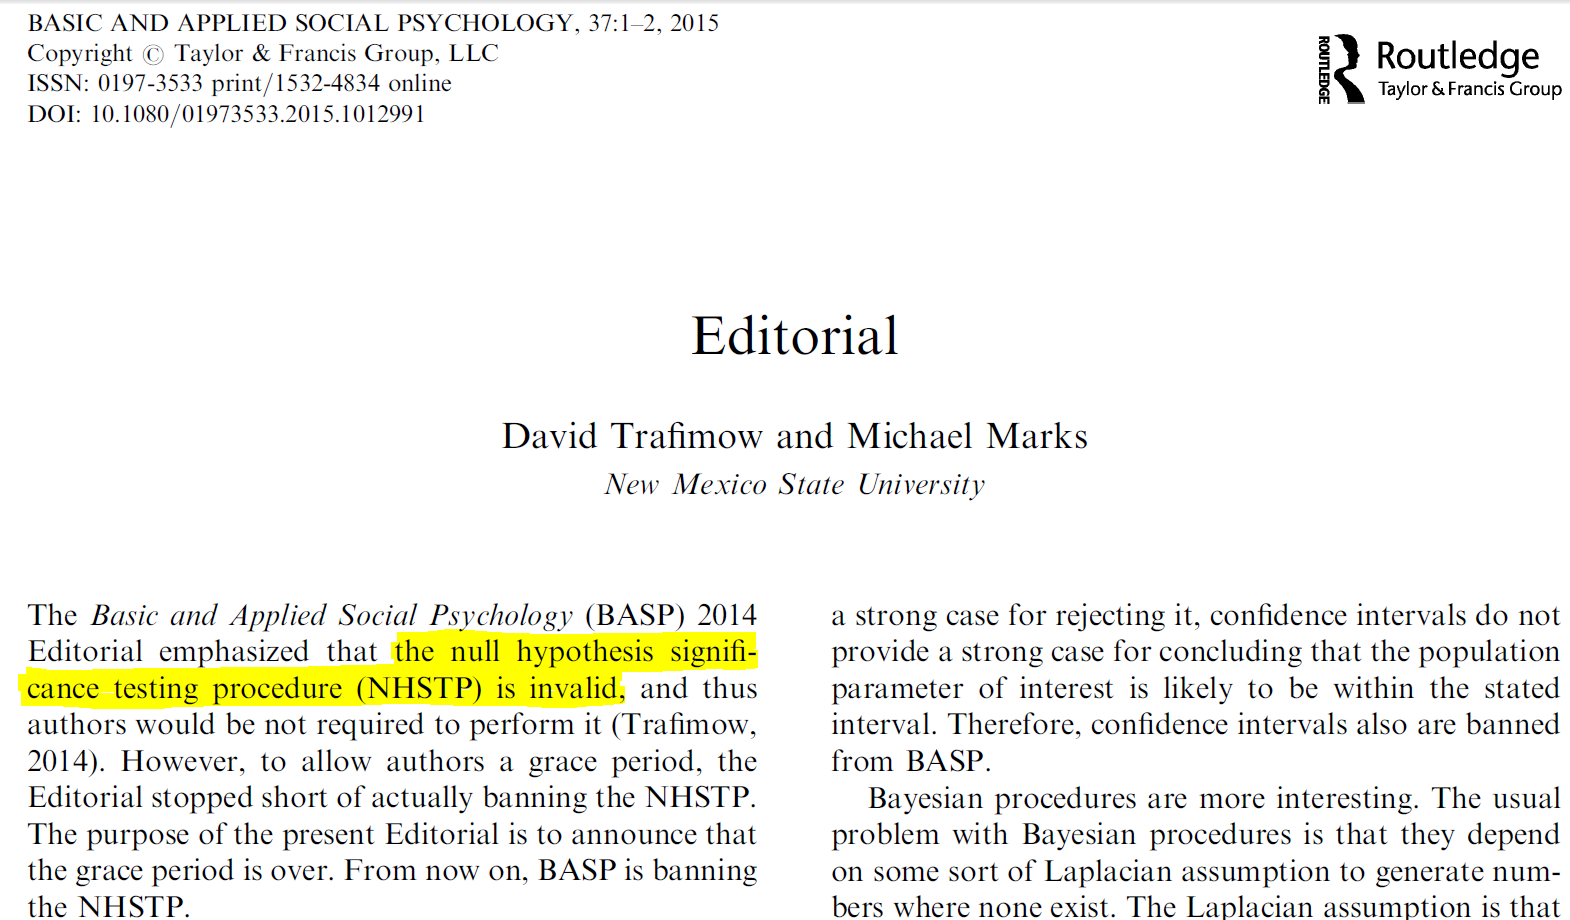
\includegraphics[width=8cm]{images/ban_editorial_1.png}
    \end{center}
  \end{overlayarea}
\end{frame}


\begin{frame}
  \frametitle{¿Por qué estoy aquí?}
  \begin{overlayarea}{\textwidth}{\textheight}
    En febrero 2015:
    \begin{center}
      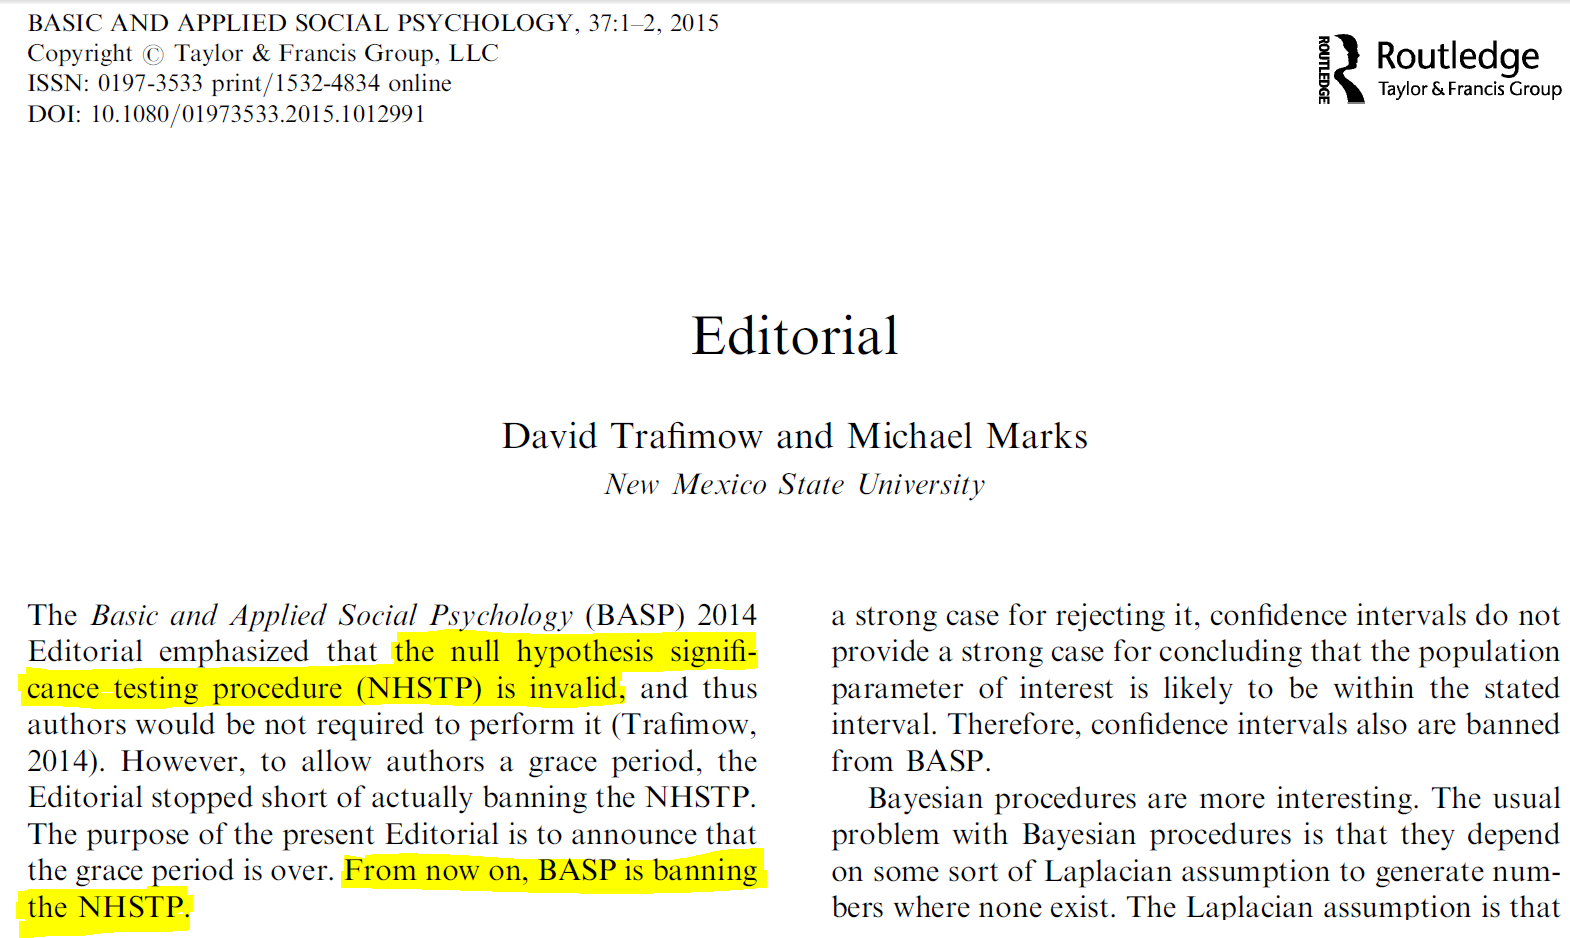
\includegraphics[width=8cm]{images/ban_editorial_2.png}
    \end{center}
    \pause
    Con Elías Moreno, un  artículo de opini\'on en BEIO:\\ 
    \textit{``It is forbidden to use p-values!''}, BEIO, 31:2, Junio
    2015.
  \end{overlayarea}
\end{frame}
\begin{frame}
  \frametitle{¿Por qué enseñamos p-valores?}

  En febrero 2014, Prof. George Cobb en un foro de discusi\'on de la
  ASA:\onslide<2->
  \begin{block}{}
    \begin{itemize}
    \item<2-> ¿Por qué se enseña $p < 0.05$ en tantos grados y
      másteres?
    \item<3-> Porque sigue siendo lo que usa la comunidad
      científica y los editores de revistas
    \item<4-> ¿Por qué sigue tanto gente usando  $p < 0.05$?
      
    \item<5-> Porque es lo que se enseña en grados y másteres.
    \end{itemize}
  \end{block}
  \onslide<6->    \hfill\begin{minipage}[h]{0.7\linewidth}
    {\scriptsize citado en \textit{R. Wassertein A. \&
        N. Lazar (2016), The American Statistician, 70:2 129-133}}
  \end{minipage}\bigskip
  
  \onslide<7->
  \begin{center}
  \Ovalbox{
    \begin{minipage}[h]{0.8\linewidth}
      \begin{itemize}
      \item   Una reflexi\'on necesaria en nuestra práctica docente.
      \item Surge también en nuestras colaboraciones con científicos aplicados. 
      \end{itemize}
      
    \end{minipage}
  }
    \end{center}
\end{frame}
\begin{frame}
  \frametitle{¿Un debate de ahora?}
  \begin{overlayarea}{\textwidth}{\textheight}
  En un seminario de Biométrica, junio 1965:
  \pause
  \begin{center}
    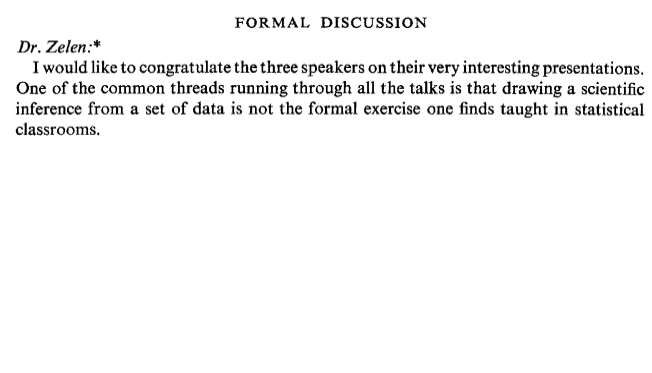
\includegraphics[width=10cm]{images/cutler_1}
  \end{center}
\end{overlayarea}
\end{frame}
\begin{frame}
    \begin{overlayarea}{\textwidth}{\textheight}
  \frametitle{¿Un debate de ahora?}
  En un seminario de Biométrica, junio 1965:
  \begin{center}
    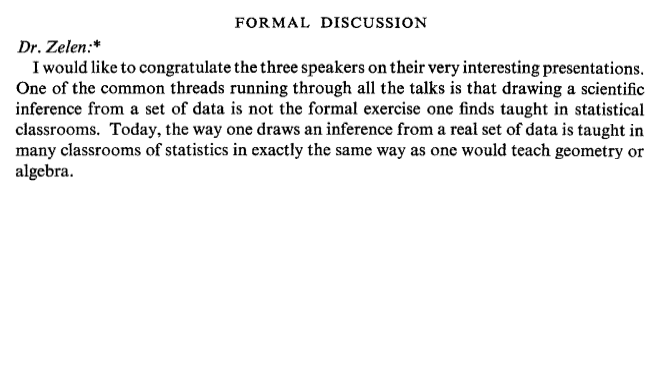
\includegraphics[width=10cm]{images/cutler_2}
  \end{center}
\end{overlayarea}
\end{frame}

\begin{frame}
  \frametitle{¿Un debate de ahora?}
    \begin{overlayarea}{\textwidth}{\textheight}
  En un seminario de Biométrica, junio 1965:
  \begin{center}
    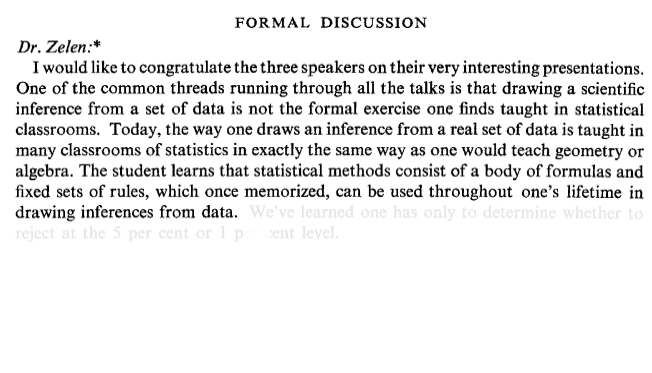
\includegraphics[width=10cm]{images/cutler_2-5}
  \end{center}
\end{overlayarea}
\end{frame}

\begin{frame}
  \frametitle{¿Un debate de ahora?}
  \begin{overlayarea}{\textwidth}{\textheight}
  En un seminario de Biométrica, junio 1965:
  \begin{center}
    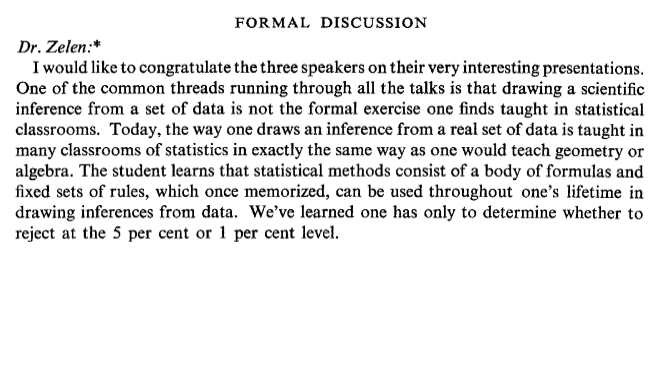
\includegraphics[width=10cm]{images/cutler_3}
  \end{center}
\end{overlayarea}
\end{frame}
\begin{frame}
  \frametitle{¿Un debate de ahora?}
    \begin{overlayarea}{\textwidth}{\textheight}
  En un seminario de Biométrica, junio 1965:
  \begin{center}
    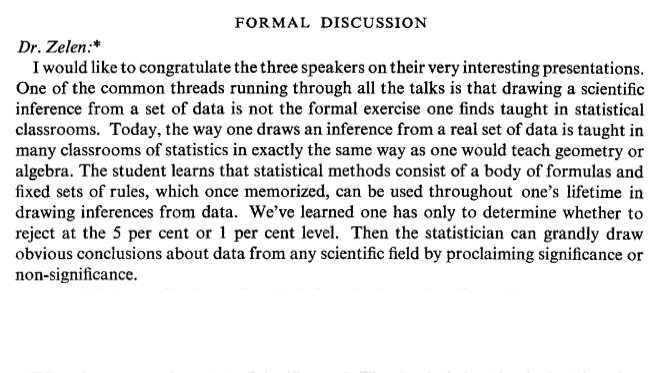
\includegraphics[width=10cm]{images/cutler_4}
  \end{center}
\end{overlayarea}
\end{frame}
\begin{frame}
  \frametitle{¿Un debate de ahora?}
    \begin{overlayarea}{\textwidth}{\textheight}
  En un seminario de Biométrica, junio 1965:
  \begin{center}
    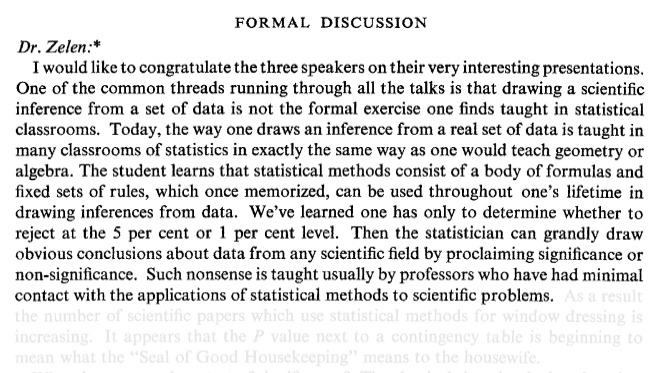
\includegraphics[width=10cm]{images/cutler_5}
  \end{center}
\end{overlayarea}
\end{frame}
\begin{frame}
  \frametitle{¿Un debate de ahora?}
    \begin{overlayarea}{\textwidth}{\textheight}
  En un seminario de Biométrica, junio 1965:
  \begin{center}
    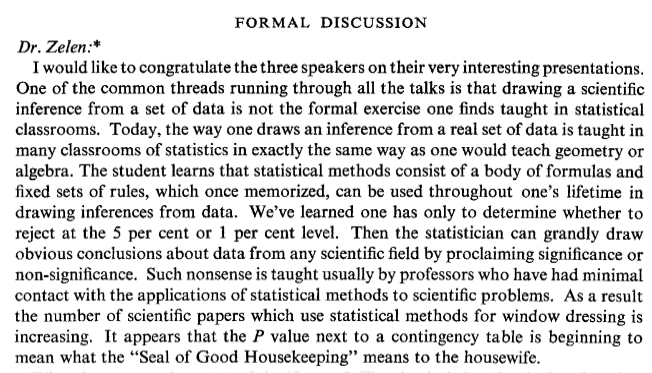
\includegraphics[width=10cm]{images/cutler_6}
  \end{center}
  \pause
  \hfill\begin{minipage}[h]{0.7\linewidth}
    {\scriptsize \textit{Cutler, S. J., Greenhouse, S. W., Cornfield, J., and Schneiderman, M. A. (1966), “The Role of Hypothesis Testing in Clinical Trials,” J Chron Disease, 19, 857–882}}
  \end{minipage}
\end{overlayarea}
\end{frame}

\begin{frame}
  \frametitle{¿Un debate de ahora?}
  En realidad desde 1930, Ha dado lugar a mucho debate y artículos,
  algunos con títulos llamativos:\bigskip\pause

  \begin{itemize}
  \item<2->  \textit{\Large The Cult of Statistical Significance: How the
      Standard Error Costs Us Jobs, Justice, and Lives.}
    \onslide<3->{\footnotesize Ziliak, S.T., and McCloskey, D.N. (2008)}\medskip
  \item<4-> \textit{\Large Significance tests as sorcery: Science is
      empirical—significance tests are not.}
    \onslide<5->{\footnotesize Lambdin (2012).}
   \end{itemize}
 \onslide<6-> En el debate, intervienen estadísticos muy relevantes. 
\end{frame}

\begin{frame}
  \frametitle{Un debate de ahora.}
Se ha avivado en los últimos años. Unos hitos:\pause

  \begin{itemize}
  \item<2->  El destierro de los p-valores de Basic Applied
    Psychology. 2015
  \item<3-> Un artículo de opinión en Nature:
    \begin{center}
      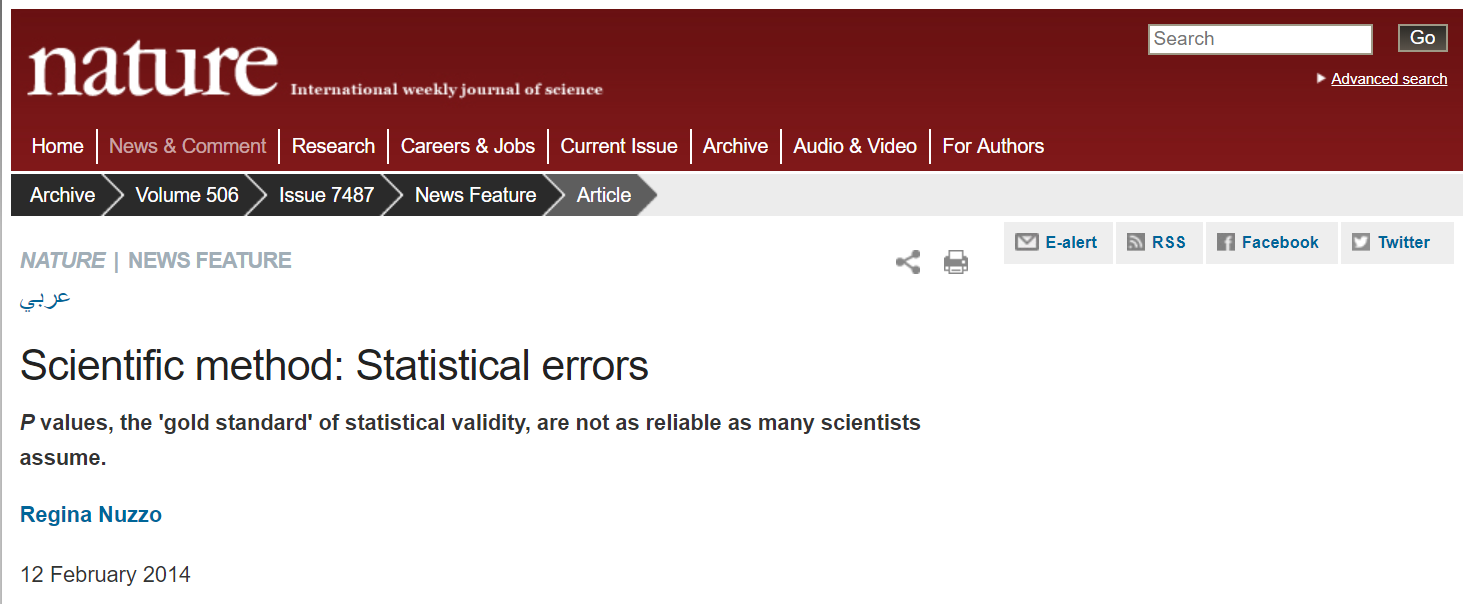
\includegraphics[width=10cm]{images/nature_nuzzo}
    \end{center}
    \onslide<4-> Uno de las más vistos en Nature de siempre.
   \end{itemize}

\end{frame}

\begin{frame}
  \frametitle{Un debate de ahora.}
  Ha llevado la American Statistical Association a emitir en 2016:\\
  \onslide<2->
  
\includegraphics[width=8cm]{images/asa_statement}\\ \onslide<3->
\hfill 
\includegraphics[width=2cm]{images/american_statistician_portada}
  \begin{itemize}
  \item<4-> Movimiento casi sin precedente en la historia de la ASA.
  \item<5-> Formaron un grupo de más de 20 expertos,
    \begin{itemize}
    \item     discusiones de
    varios meses,
  \item  un meeting de 2 días, 
  \item varios borradores hasta la
    aprobación del texto final.
    \end{itemize}
  \end{itemize}
 
\end{frame}
\begin{frame}
  \frametitle{Un debate de ahora.}
  A continuación organizaron en 2017
   \onslide<2->
  
\includegraphics[width=8cm]{images/asa_symposium}\\ \onslide<3->
  Asociado a este symposium un \href{https://www.tandfonline.com/toc/utas20/73/sup1}{número especial} de The American
  Statistician:\onslide<4->

  \begin{center}
    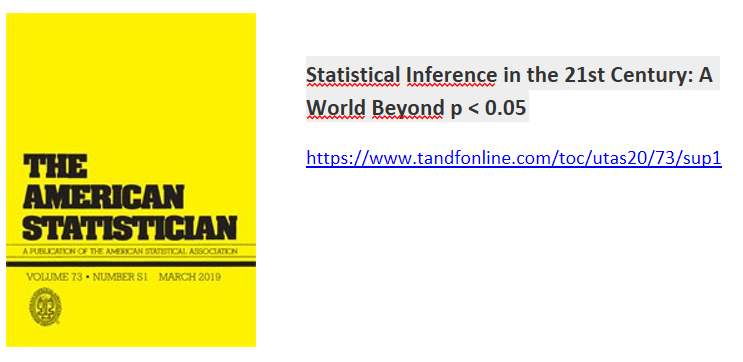
\includegraphics[width=8cm]{images/asa_special_issue}
  \end{center}
 
\end{frame}
\begin{frame}
  \frametitle{Un debate de ahora.}
  A continuación organizaron en 2017
  
\includegraphics[width=8cm]{images/asa_symposium}\\ 
  Asociado a este symposium un número especial de The American
  Statistician:

  \begin{center}
    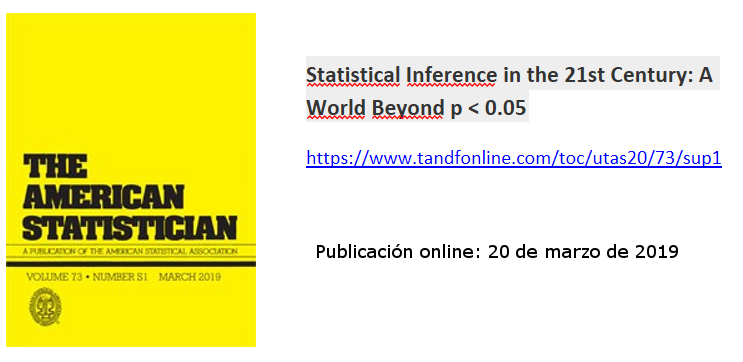
\includegraphics[width=8cm]{images/asa_special_issue_2}
  \end{center}
 
\end{frame}

\begin{frame}
  \frametitle{Un debate de ahora.}
  A la misma vez, en Nature:\\ \onslide<2->
  \begin{center}
  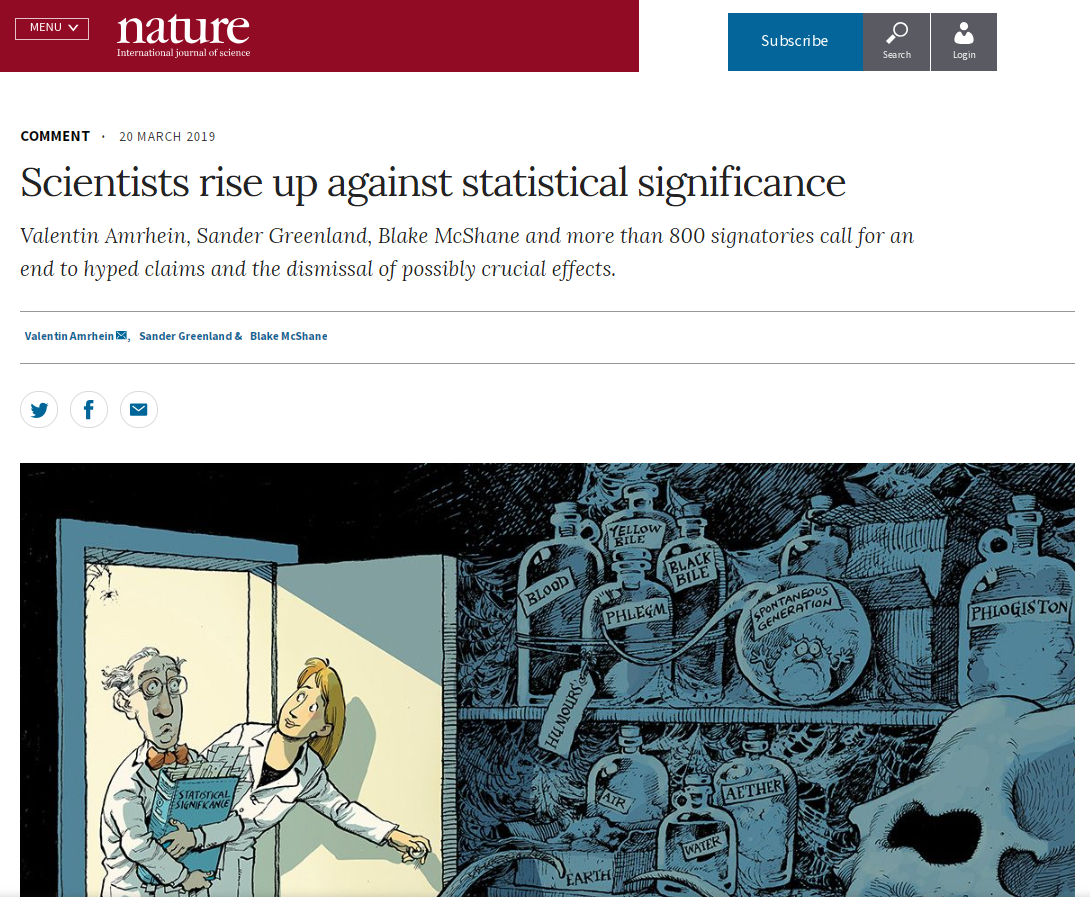
\includegraphics[width=10cm]{images/nature_amrhein}
  \end{center}
\end{frame}


\begin{frame}
  \frametitle{Un debate de ahora.}
  En este podcast recomendable:\\ \onslide<2->
  \begin{center}
  
\includegraphics[width=10cm]{images/nssd_1}
  \end{center}
\end{frame}


\begin{frame}
  \frametitle{Un debate de ahora.}
  En este podcast recomendable:\\ 
  \begin{center}
  
\includegraphics[width=10cm]{images/nssd_2}
  \end{center}
\end{frame}


\begin{frame}
  \frametitle{Un debate de ahora.}
  En este podcast recomendable:\\ 
  \begin{center}
  
\includegraphics[width=10cm]{images/nssd_3}
  \end{center}
\end{frame}

\begin{frame}
  \frametitle{Un debate de ahora.}
  Y además, en cuanto a enseñanza\\ \onslide<2->
  \begin{center}
  
\includegraphics[width=8cm]{images/USCOTS}
  \end{center}
\end{frame}


\begin{frame}
  \frametitle{¿Por qué tanto ataque a los p-valores?}
  \onslide<2-> Se enmarca en la llamada\\
    \begin{center}
  \Ovalbox{\Huge Crisis de la reproducibilidad}
\end{center}
\onslide<3->
\begin{block}{A veces se distinguen dos términos:}
  \begin{itemize}
    \item \textbf{Replicabilidad:} relacionado a las posibilidades de que un
    experimento independiente que busque contestar a la misma pregunta
    científica confirme los resultados.
  \item \textbf{Reproducibilidad:} capacidad de reproducir
    el análisis de datos a partir de los datos originales, y el
    conocimiento de flujo de manipulación y análisis. 
  \end{itemize}
  
\end{block}
\end{frame}

\begin{frame}
  \frametitle{La crisis de la reproducibilidad}
  \onslide<2-> Algunos ejemplos con impacto\\
  \begin{block}{2006: \textit{Nature Medicine}}
    El equipo de A. Potti en Duke publican un algoritmo que predice, a
    partir de datos de chips ADN, qué pacientes de cáncer responderán
    a la quimioterapia.
  \end{block}
      \onslide<3->
      \begin{itemize}
      \item<3-> Gran repercusión
      \item<4-> Datos públicos, dos estadísticos Baggerly \& Coombes
        intentan aplicar los algoritmos
        
      \item<5-> Encontraton muchos errores, desde triviales a muy
        graves
      \item<6-> Fueron incluso capaces de reproducir el análisis
        erróneo
      \item<7-> Fue retirado de la revista en 2011.   
      \end{itemize}
\end{frame}

\begin{frame}
  \frametitle{La crisis de la reproducibilidad}
  \begin{center}
    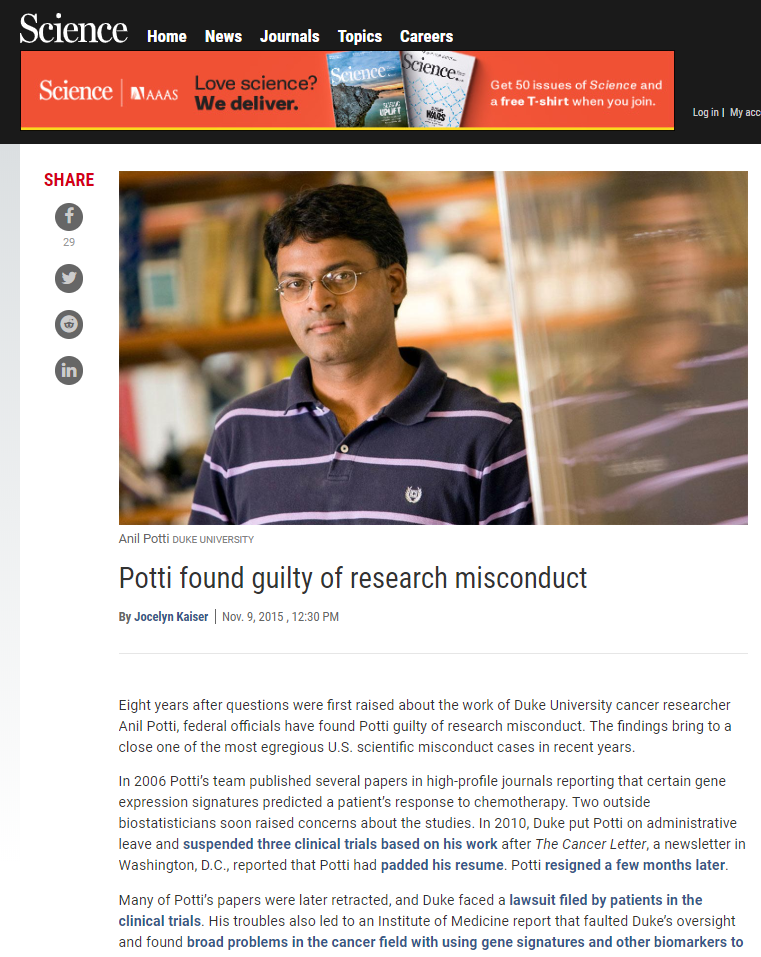
\includegraphics[height=0.85\textheight]{images/potti_portada_1}
  \end{center}
  \hfill\begin{minipage}[h]{0.8\linewidth}
    {\tiny \textit{https://www.sciencemag.org/news/2015/11/potti-found-guilty-research-misconduct}}
  \end{minipage}
\end{frame}

\begin{frame}
  \frametitle{La crisis de la reproducibilidad}
  \begin{center}
    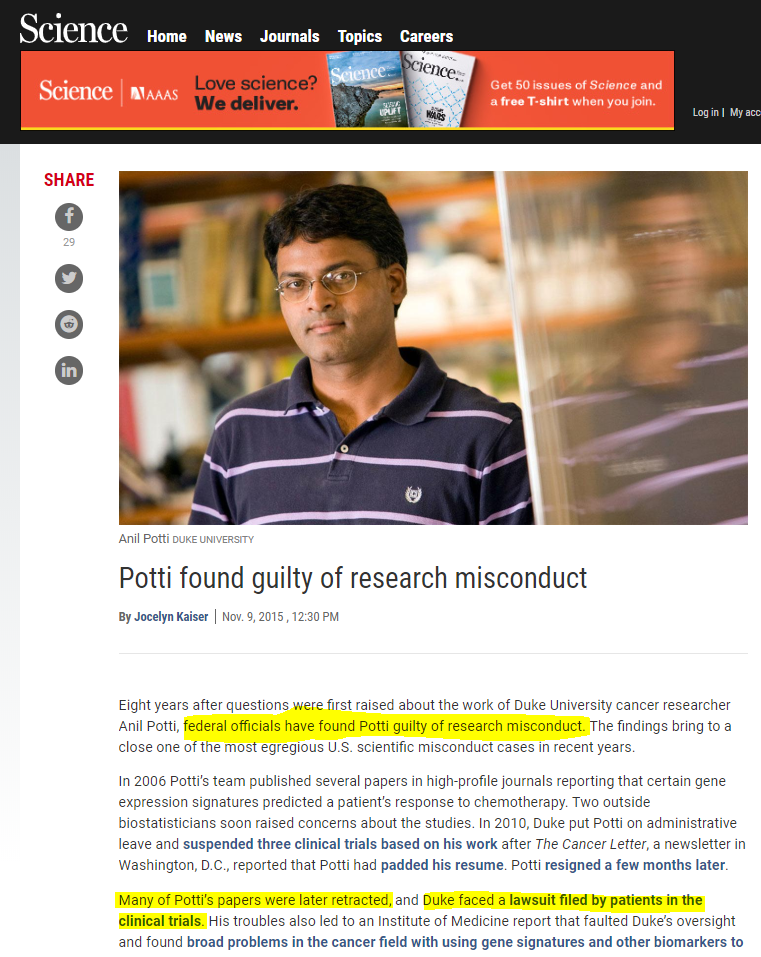
\includegraphics[height=0.85\textheight]{images/potti_portada_2}
  \end{center}
    \hfill\begin{minipage}[h]{0.8\linewidth}
    {\tiny \textit{https://www.sciencemag.org/news/2015/11/potti-found-guilty-research-misconduct}}
  \end{minipage}
\end{frame}

\begin{frame}
  \frametitle{La crisis de la reproducibilidad}
  \begin{center}
    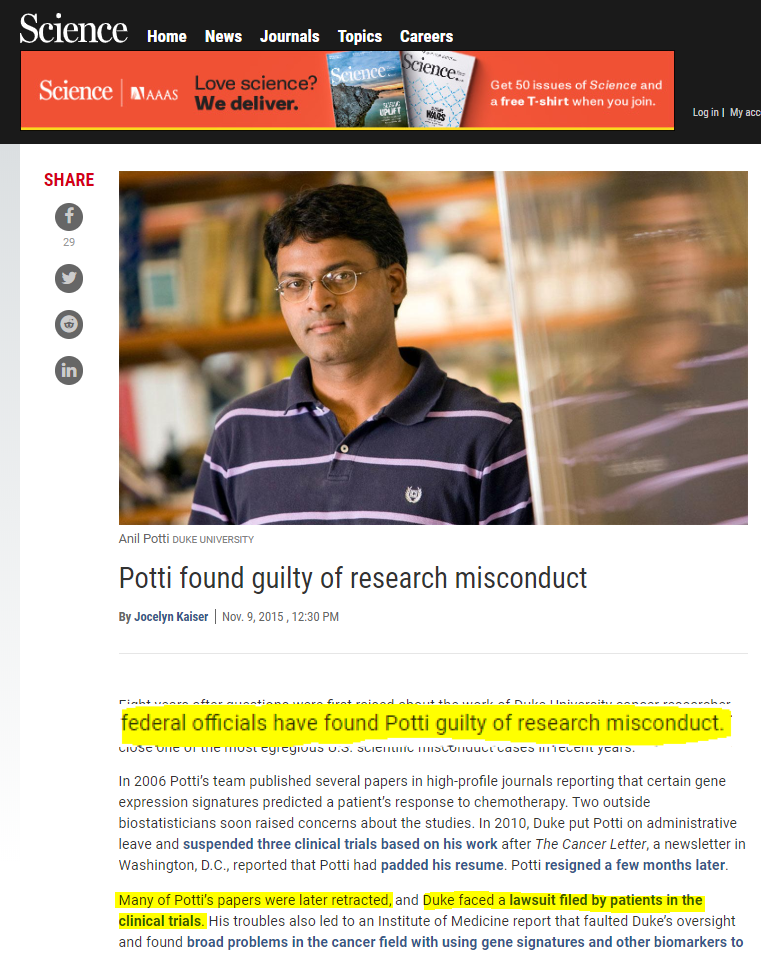
\includegraphics[height=0.85\textheight]{images/potti_portada_3}
  \end{center}
  \hfill\begin{minipage}[h]{0.8\linewidth}
    {\tiny \textit{https://www.sciencemag.org/news/2015/11/potti-found-guilty-research-misconduct}}
  \end{minipage}
\end{frame}

\begin{frame}
  \frametitle{La crisis de la reproducibilidad}
  \begin{center}
    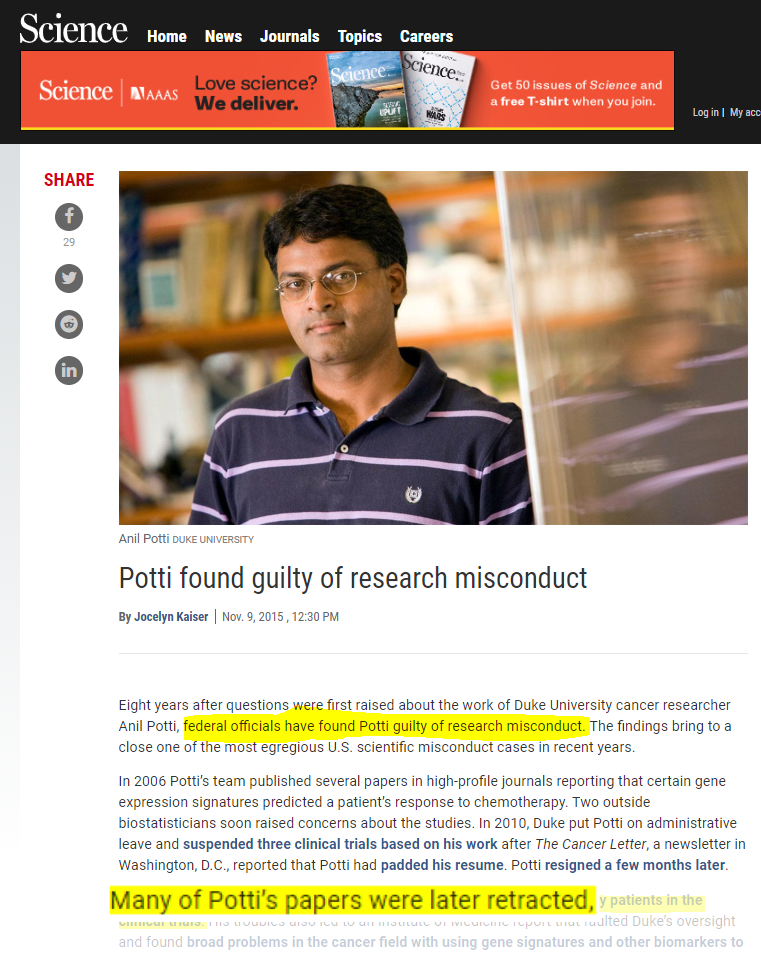
\includegraphics[height=0.85\textheight]{images/potti_portada_4}
  \end{center}
  \hfill\begin{minipage}[h]{0.8\linewidth}
    {\tiny \textit{https://www.sciencemag.org/news/2015/11/potti-found-guilty-research-misconduct}}
  \end{minipage}
\end{frame}

\begin{frame}
  \frametitle{La crisis de la reproducibilidad}
  \begin{center}
    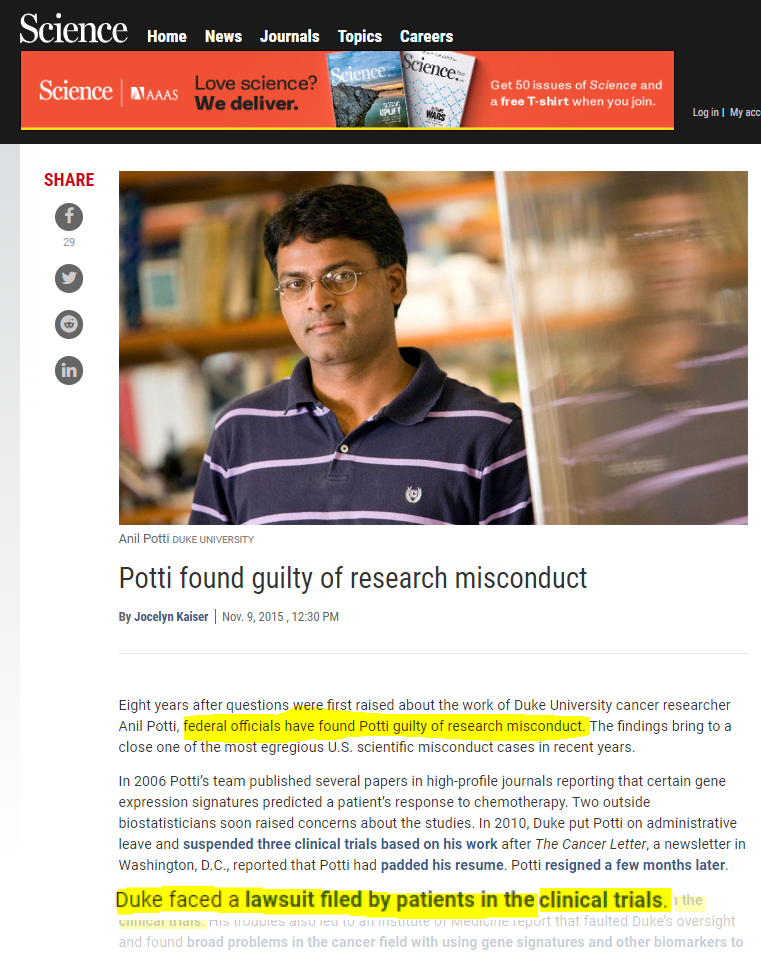
\includegraphics[height=0.85\textheight]{images/potti_portada_5}
  \end{center}
  \hfill\begin{minipage}[h]{0.8\linewidth}
    {\tiny \textit{https://www.sciencemag.org/news/2015/11/potti-found-guilty-research-misconduct}}
  \end{minipage}
\end{frame}

\begin{frame}
  \frametitle{La crisis de la reproducibilidad}
  
  \begin{center}
    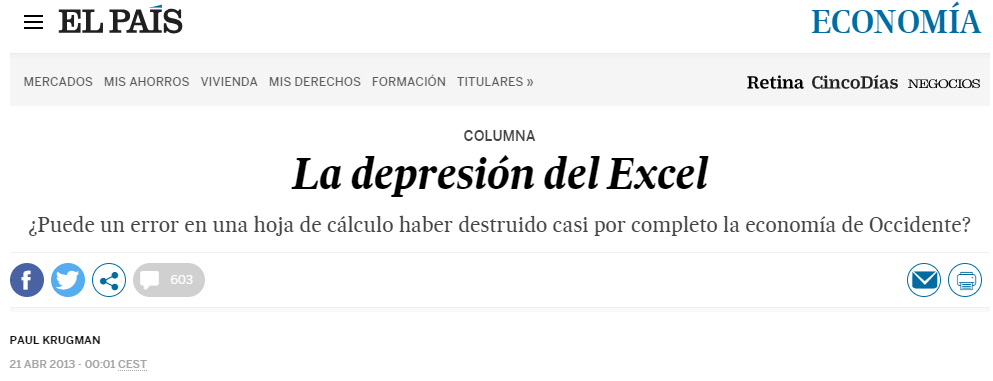
\includegraphics[width=0.8\textwidth]{images/elpais_krugman}
  \end{center}
  \onslide<2->
  \begin{block}{2010, \textit{the National Bureau of Economic Research}}
  2010, Carmen Reinhart \& Kenneth Rogoff, Harvard, publican \textit{``Growth in a time
    of debt''}.
  \onslide<3-> Aseguraron que países con $Deuda / PIB$ altos sufrían
  bajo crecimiento, identificando incluso el umbral 90\%.
\end{block}
\begin{itemize}
  \scriptsize
  \item<4-> Inmediatamente críticas: por una parte por llevar a
    confundir asociación y causalidad. 
  \item<5-> Porque otros, partiendo de datos similares, no pudieron reproducir
    los resultados.
  \item<6-> Por la presión, publicaron el Excel.
  \item<7->  Thomas Herndon, estudiante de grado economía, encontró
    varios errores: un error fórmula Excel, ponderaciones no estándar.
  \end{itemize}
\end{frame}


\begin{frame}
  \frametitle{La crisis de la reproducibilidad}
  En \textit{Science}, 2015, 270 autores  Open Science
  Collaboration:\\ \onslide<2->
  \textbf{Estimating the reproducibility of psychological science}.\\
  Prueban a replicar 100 experimentos en 3 revistas de psicología. \\
  \onslide<3-> Originales: 97\% estad.
  significativos. Réplicas: 36\% estad. significativos.\onslide<4->
  \begin{center}
    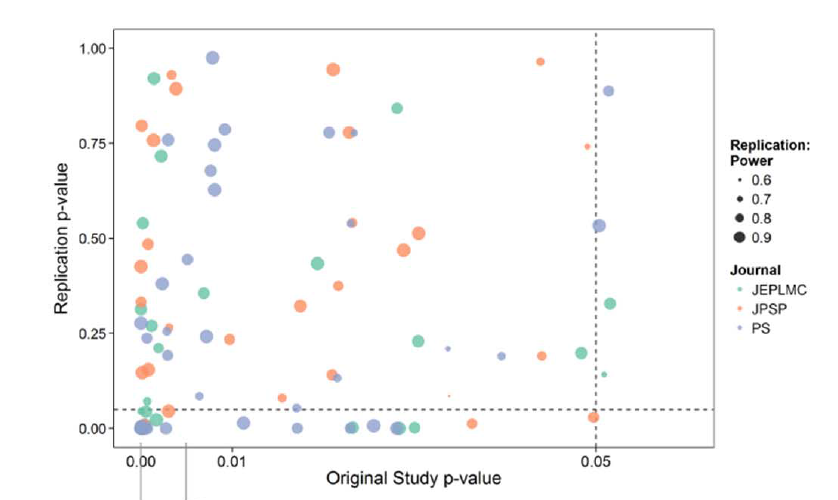
\includegraphics[width=0.8\textwidth]{images/original_vs_replicated_p-value}
  \end{center}
\end{frame}

\begin{frame}
  \frametitle{La crisis de la reproducibilidad}
  \begin{overlayarea}{\textwidth}{\textheight}
  \begin{center}
    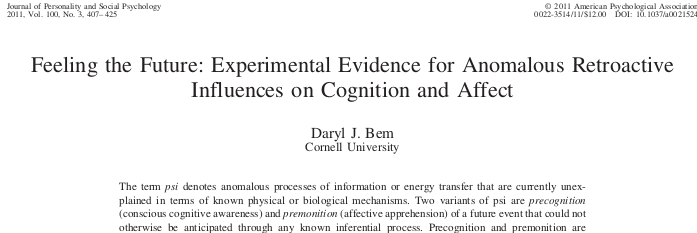
\includegraphics[width=0.8\textwidth]{images/bem}
  \end{center}\onslide<2->
  \begin{block}{Extra Sensory Perception (ESP)}
    Nueve experimentos. \\
    \onslide<3->
    E.g el experimento 1:
    \begin{itemize}
    \item<3-> los participantes
tenían que adivinar si una imagen iba a aparecer a la izquierda o
derecha de la pantalla.
    
\item<4-> Bem encuentra que, si se trata de imágenes eróticas,
  aciertan con más frecuencia que si fuera al azar. 
    \end{itemize}
    
  \end{block}
\end{overlayarea}  

\end{frame}


\begin{frame}
  \frametitle{La crisis de la reproducibilidad}
  \begin{overlayarea}{\textwidth}{\textheight}
  \begin{center}
    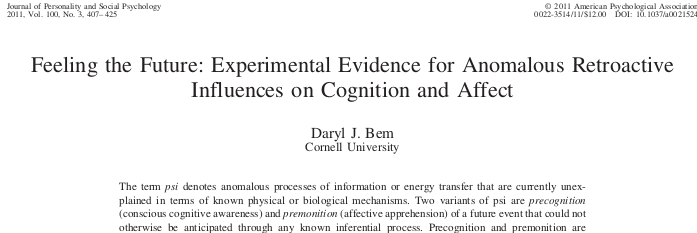
\includegraphics[width=0.8\textwidth]{images/bem}
  \end{center}
\begin{center}
    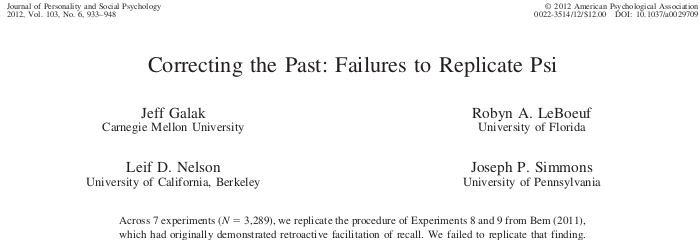
\includegraphics[width=0.8\textwidth]{images/failure_to_replicate_bem}
  \end{center}
\end{overlayarea}
\end{frame}

\begin{frame}
  \frametitle{La crisis de la reproducibilidad}
    \begin{overlayarea}{\textwidth}{\textheight}
  ¿Son casos aislados?\\ \onslide<2->
    \begin{center}
    
\includegraphics[width=0.8\textwidth]{images/nature_irreproducible_research}
  \end{center}
\onslide<3->
Nature realiza una encuesta a 1500 investigadores:
\begin{center}
\begin{block}{}
    \begin{itemize}
    \item<4-> El 70\% no consiguió en alguna ocasión replicar experimentos de otros.
    \item<4-> Más del 50\% no consiguió en alguna ocasión replicar sus propios experimentos.
    \end{itemize}
  \end{block}
\end{center}
\end{overlayarea}
\end{frame}

\begin{frame}
  \frametitle{La crisis de la reproducibilidad}
    \begin{overlayarea}{\textwidth}{\textheight}
  ¿Son casos aislados?\\ 
    \begin{center}
    
\includegraphics[width=0.8\textwidth]{images/nature_irreproducible_research}
  \end{center}
Identifican tres ámbitos
\begin{center}
\Ovalbox{\Large Experimental, computacional, estadístico}
\end{center}
\end{overlayarea}
\end{frame}

\begin{frame}
  \frametitle{La crisis de la reproducibilidad}
    \begin{overlayarea}{\textwidth}{\textheight}
  Una manera poderosa de reducir la irreproducibilidad es fomentar la
  ciencia abierta\vspace{-0.5cm}\\ \onslide<2->
    \begin{center}
    
\includegraphics[width=0.8\textwidth]{images/science_as_open_enterprise}
  \end{center}\vspace{-0.5cm}
\hfill {\tiny \href{https://royalsociety.org/topics-policy/projects/science-public-enterprise/report/}{https://royalsociety.org/topics-policy/projects/science-public-enterprise/report/}}\onslide<3->
  \begin{center}
    \Ovalbox{\Large  \begin{minipage}[h]{1.0\linewidth}
           Open\ Science  =  Open\ Data  + \\
          \hphantom{ Open\ Acess  =  Open\ }Open\ Access\ to \ scientific\ publications +\\
          \hphantom{ Open\ Acess  =  Open\ Open\ }effective\ communication.
       \end{minipage}
      
    }
      
\end{center}
\end{overlayarea}
\end{frame}

\begin{frame}
  \frametitle{La crisis de la reproducibilidad}
    \begin{overlayarea}{\textwidth}{\textheight}
     \begin{center}
    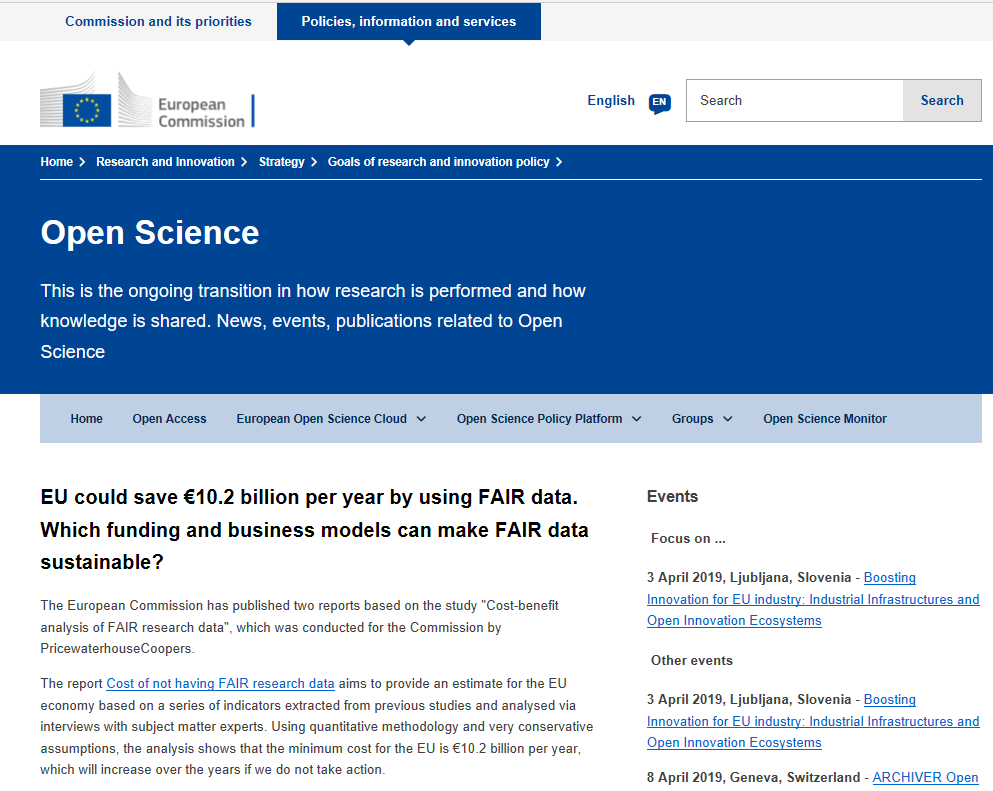
\includegraphics[width=0.8\textwidth]{images/open_science_EU}
  \end{center}\vspace{-0.5cm}
\hfill {\scriptsize \href{https://ec.europa.eu/research/openscience/index.cfm}{https://ec.europa.eu/research/openscience/index.cfm}}\onslide<2->
  \begin{center}
    \Ovalbox{\Large  
           FAIR  =  Findable  + Accesible + Interoperable + Reusable
    }
    
\end{center}
\end{overlayarea}
\end{frame}

\begin{frame}
  \frametitle{¿Qué papel juegan los $p$-valores en esta crisis?}
 ¿Qué parte de culpa tienen? \medskip\\ \onslide<+->
 Los $p$-valores llevan muchos años en la piqueta.\onslide<+-> \\
 Un investigador incluso propuso cambiarle el nombre a\onslide<+->
 \begin{center}
   \Ovalbox{\large Statistical Hypothesis Inference Testing}
 \end{center}\onslide<+->
 por el acrónimo... \onslide<+->  \hfill {\tiny Citado en Nuzzo (2014) \href{https://www.nature.com/news/scientific-method-statistical-errors-1.14700}{enlace}}
\bigskip \\
 \onslide<+-> Se ha establecido
 \begin{align*}
 Statistical\ Significance &\Leftrightarrow Scientific\
                             Significance.\\
   \onslide<+->{  Statistical\ Significance &\Leftrightarrow p < 0.05\\}
    \onslide<+->{  Scientific\ Significance &\Leftrightarrow p < 0.05}
 \end{align*}
\end{frame}
\begin{frame}
  \frametitle{¿Qué papel juegan los $p$-valores en esta crisis?}
  Por cierto, ¿dónde aparece $p < 0.05$?\onslide<2->
 \begin{center}
    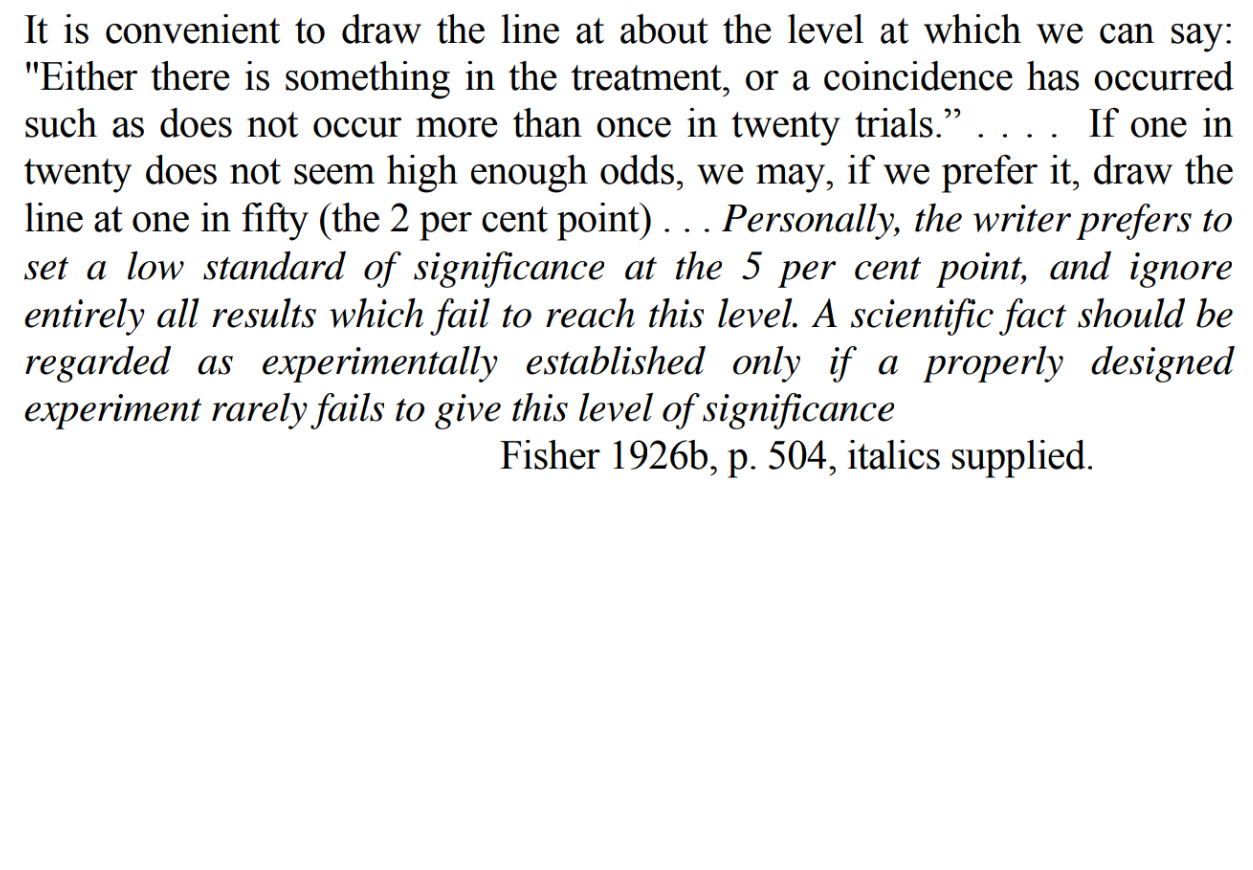
\includegraphics[width=10cm]{images/fisher_p-value_0.png}
  \end{center}
  \hfill
    {\scriptsize \textit{S. Ziliak \& D. McCloskey(2009) ``The Cult of
        Statistical Significance''. JSM 2009, \href{https://www.deirdremccloskey.com/docs/jsm.pdf}{enlace}}}
  \end{frame}

\begin{frame}
  \frametitle{¿Qué papel juegan los $p$-valores en esta crisis?}
  Por cierto, ¿dónde aparece $p < 0.05$?
 \begin{center}
    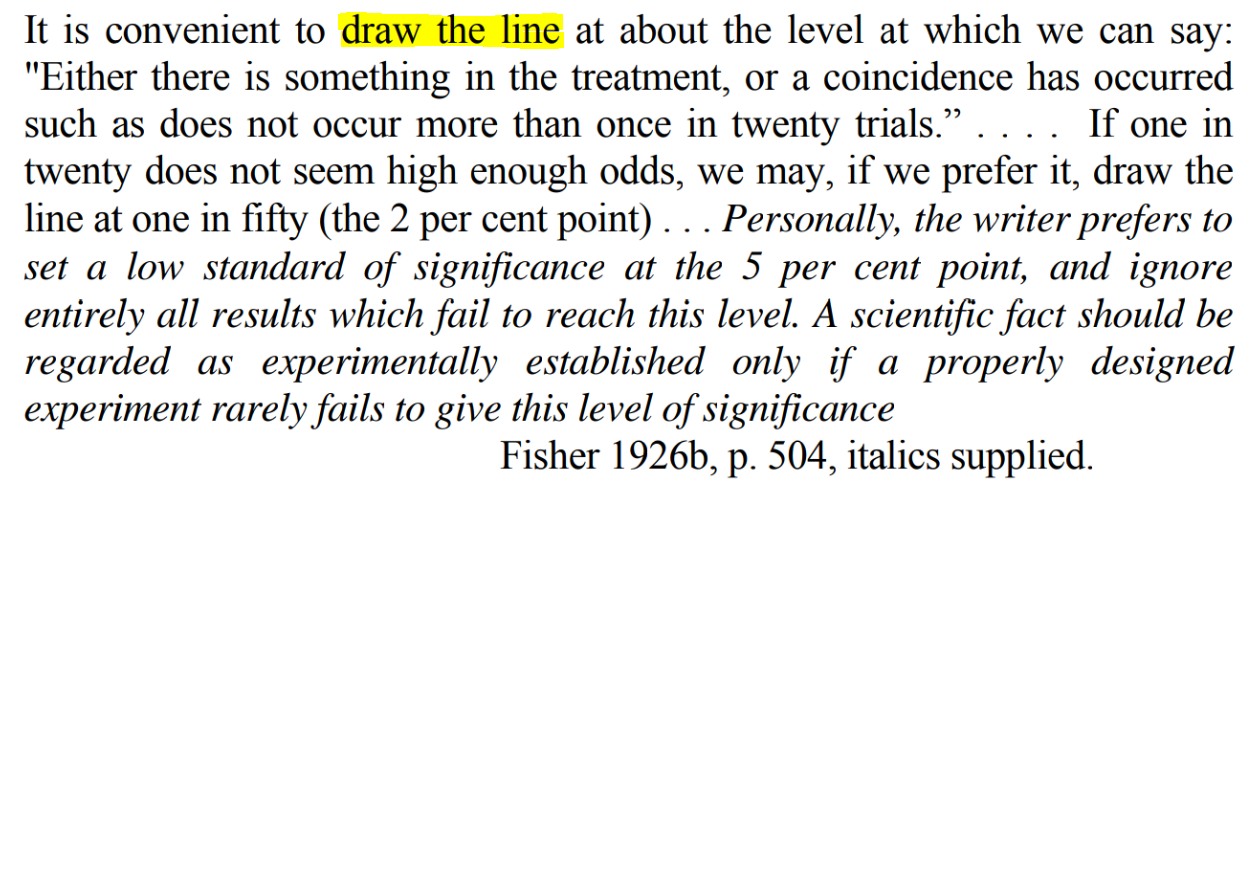
\includegraphics[width=10cm]{images/fisher_p-value_1.png}
  \end{center}
  \hfill
    {\scriptsize \textit{S. Ziliak \& D. McCloskey(2009) ``The Cult of
        Statistical Significance''. JSM 2009, \href{https://www.deirdremccloskey.com/docs/jsm.pdf}{enlace}}}
\end{frame}


\begin{frame}
  \frametitle{¿Qué papel juegan los $p$-valores en esta crisis?}
  Por cierto, ¿dónde aparece $p < 0.05$?
 \begin{center}
    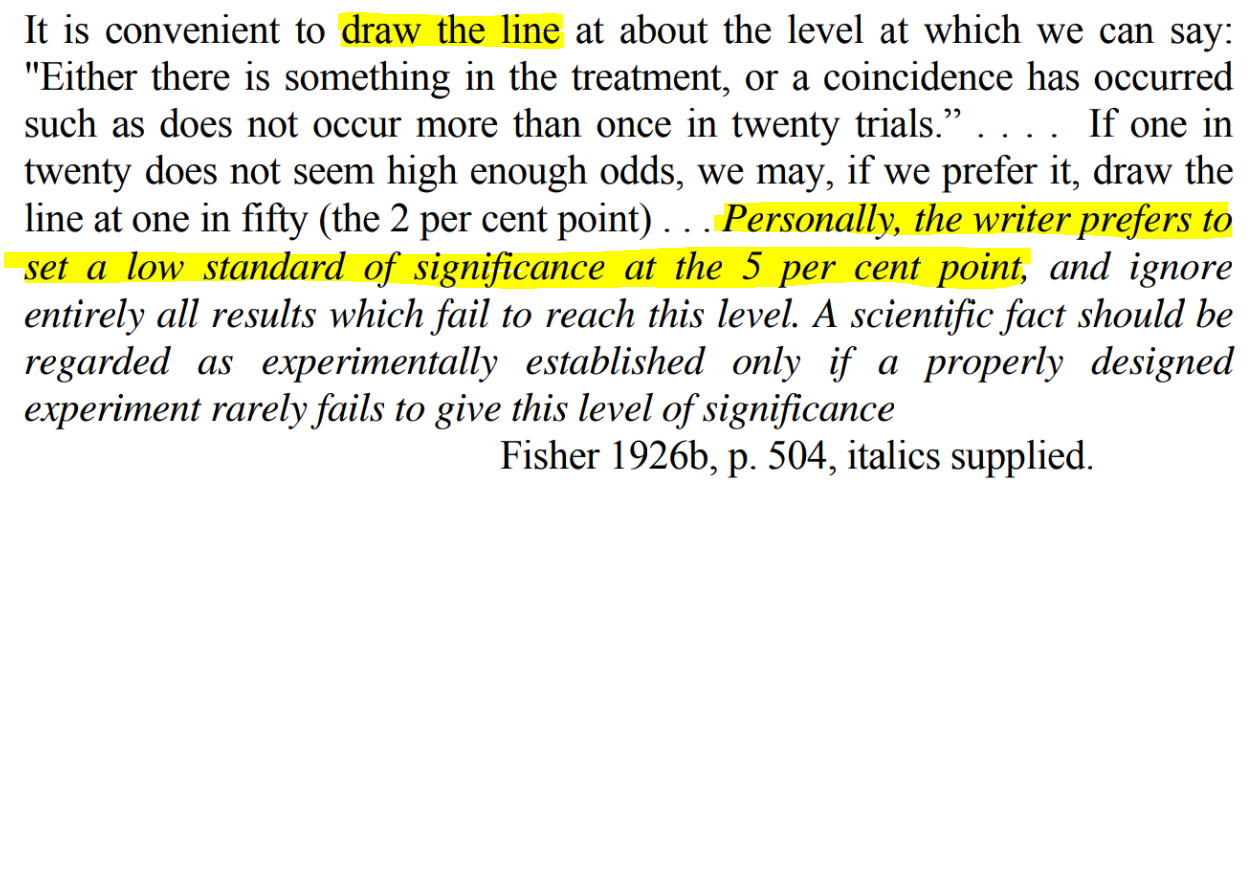
\includegraphics[width=10cm]{images/fisher_p-value_2.png}
  \end{center}
  \hfill
    {\scriptsize \textit{S. Ziliak \& D. McCloskey(2009) ``The Cult of
        Statistical Significance''. JSM 2009, \href{https://www.deirdremccloskey.com/docs/jsm.pdf}{enlace}}}
\end{frame}


\begin{frame}
  \frametitle{¿Qué papel juegan los $p$-valores en esta crisis?}
  Por cierto, ¿dónde aparece $p < 0.05$?
 \begin{center}
    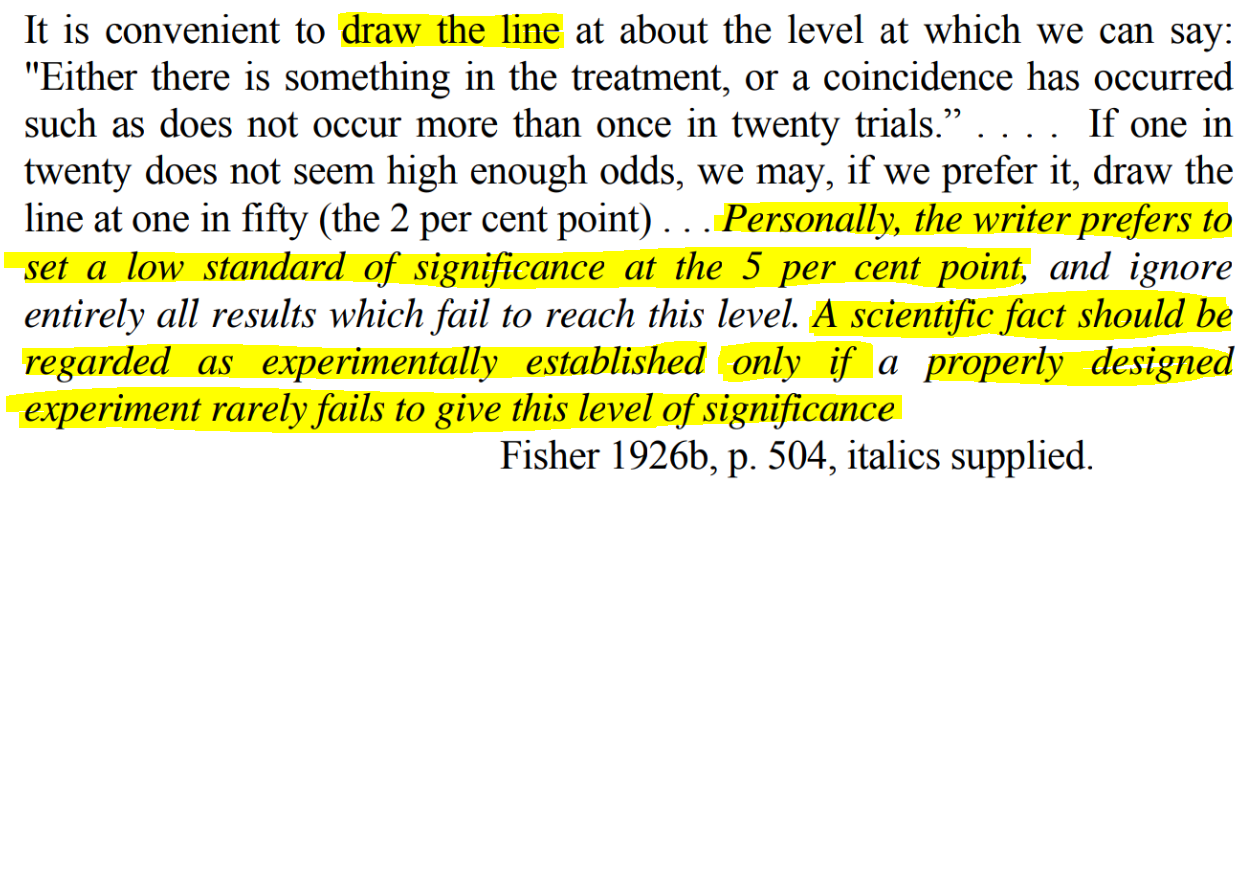
\includegraphics[width=10cm]{images/fisher_p-value_2-5.png}
 \end{center}\hfill
    {\scriptsize \textit{S. Ziliak \& D. McCloskey(2009) ``The Cult of
        Statistical Significance''. JSM 2009, \href{https://www.deirdremccloskey.com/docs/jsm.pdf}{enlace}}}
\end{frame}

\begin{frame}
  \frametitle{¿Qué papel juegan los $p$-valores en esta crisis?}
  Por cierto, ¿dónde aparece $p < 0.05$?
 \begin{center}
    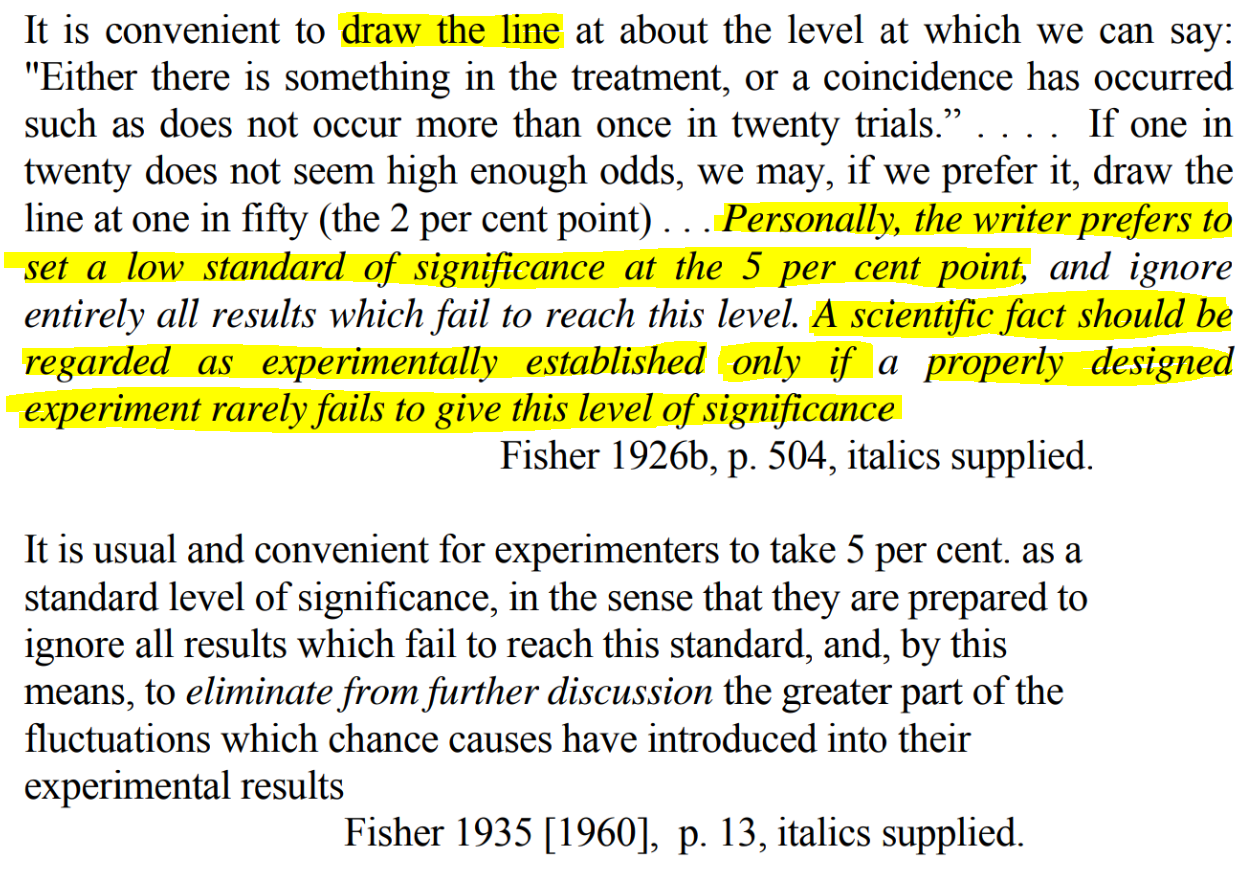
\includegraphics[width=10cm]{images/fisher_p-value_3.png}
 \end{center}\hfill
    {\scriptsize \textit{S. Ziliak \& D. McCloskey(2009) ``The Cult of
        Statistical Significance''. JSM 2009, \href{https://www.deirdremccloskey.com/docs/jsm.pdf}{enlace}}}
\end{frame}


\begin{frame}
  \frametitle{¿Qué papel juegan los $p$-valores en esta crisis?}
  ¿Están efectivamente muy usados en la investigación científica?
  \onslide<+->

  \begin{block}{}
    John Ioannidis, Stanford, y colaboradores han estudiado en muchos
    artículos la presencia de $p$-valores a través de minería de textos
    en las bases de datos bibliográficas
  \end{block}
  \onslide<+-> En su \href{https://doi.org/10.1080/00031305.2018.1447512}{contribución} al volumen especial de \textit{The
    American Statistician}, 2019:
  \begin{itemize}
  \item<+-> Analizan  13 millones de abstracts y 844\,000 artículos
    completos de PubMed Central.
  \item<+-> 51\% de los abstracts contienen un $p$-valor.
  \item<+-> Entre los que contienen un $p$-valor, el 96\% tienen
    $p<0.05$.
  \item<+-> Entre 1990 y 2015, la presencia de $p$-valores se ha
    multiplicado por dos en los abstracts analizados. 
  \end{itemize}\bigskip
  \onslide<+->

  \begin{center}
      \Ovalbox{\textit{``Too good to be true?''}}
  \end{center}
  \onslide<+-> En 2005:
   Ioannidis JPA (2005) ``Why Most Published Research Findings Are False.'' \textit{PLOS Medicine} 2(8): e124.
\end{frame}

\begin{frame}
  \frametitle{¿Qué papel juegan los $p$-valores en esta crisis?}
    \begin{overlayarea}{\textwidth}{0.8\textheight}
  Vamos a hablar de tres problemas, que pueden juegar un
  papel.\vspace{1cm}
  \onslide<+->
  \begin{center}
    \Ovalbox{
      \begin{minipage}[h]{0.9\linewidth}
  \begin{enumerate}
    \Large
  \item<+-> Las dificultades de interpretación del $p$-valor propician
    la confusión $p<0.05\Leftrightarrow Scientific\ significance$.\medskip
  \item<+-> La elección del umbral $p = 0.05$. \medskip
  \item<+-> La existencia del ``$p$-hacking''. 
  \end{enumerate}
\end{minipage}
}
  \end{center}
\end{overlayarea}
\end{frame}



\begin{frame}
  \frametitle{Primer problema: interpretación del $p$-valor}
    \begin{overlayarea}{\textwidth}{0.8\textheight}
  Un hecho innegable:\medskip \onslide<+->

  \begin{center}
  \Ovalbox{\Huge El $p$-valor se presta a interpretaciones erróneas}    
  \end{center}\medskip

En, por ejemplo,
\begin{itemize}
\item Ronald L. Wasserstein \& Nicole A. Lazar (2016) The ASA's
  Statement on p-Values: Context, Process, and Purpose, \textit{The
    American Statistician}, 70:2, 129-133.\href{https://doi.org/10.1080/00031305.2016.1154108}{enlace}
\item Ronald L. Wasserstein, Allen L. Schirm \& Nicole A. Lazar (2019)
  Moving to a World Beyond ``$p < 0.05$'', \textit{The American
    Statistician}, 73:sup1, 1-19. \href{https://doi.org/10.1080/00031305.2019.1583913}{enlace}
\item Greenland, S., Senn, S.J., Rothman, K.J. et al.(2016)  ``Statistical tests, P values, confidence intervals, and power: a guide to misinterpretations''. \textit{Eur J Epidemiol}  31: 337. \href{https://doi.org/10.1007/s10654-016-0149-3}{enlace}.
\end{itemize}
se enfatiza lo que \textbf{NO} es un $p$-valor.
\end{overlayarea}
\end{frame}

\begin{frame}
  \frametitle{Primer problema: interpretación del $p$-valor}
    \begin{overlayarea}{\textwidth}{0.8\textheight}
El $p$-valor no es la probabilidad de que la hipótesis nula sea cierta
basado en mis datos observados!!!!\onslide<2->

\begin{center}
  \Ovalbox{
    \begin{minipage}[h]{0.8\linewidth}
      El $p$-valor sí es una medida de la compatibilidad de los datos
observados con el modelo 
\only<2>{completo}\onslide<3->{\alert{completo}}
    \end{minipage}
  }
\end{center}

\onslide<4->
Por lo tanto:
\begin{itemize}
\item<5-> El $p$-valor no es un indicador sólamente de la evidencia presente en
los datos sobre si $H_0$ es verdadera, sino que depende evidentemente
de todas las hipótesis realizadas en la construcción del
modelo.
\item<6-> En esta compatibilidad de los datos observados con el modelo
  completo, entra todo.
\item<7-> Cualquier valor del efecto que lleva a un $p$-valor mayor
  que el observado, es más compatible con los datos observados. 
\end{itemize}

\end{overlayarea}
\end{frame}

\begin{frame}
  \frametitle{Primer problema: interpretación del $p$-valor}
    \begin{overlayarea}{\textwidth}{0.8\textheight}
  Un hecho innegable:\medskip \onslide<+->

  \begin{center}
  \Ovalbox{\Huge El $p$-valor se presta a interpretaciones erróneas}    
  \end{center}\medskip

  El artículo pedagógico
  \begin{itemize}
  \item  Greenland, S., Senn, S.J., Rothman, K.J. et al.(2016)  ``Statistical tests, P values, confidence intervals, and power: a guide to misinterpretations''. \textit{Eur J Epidemiol}  31: 337. \href{https://doi.org/10.1007/s10654-016-0149-3}{enlace}.
\end{itemize}\bigskip \onslide<+->
 \begin{center}
   \Huge \href{https://play.kahoot.it/v2/?quizId=4a06411c-9dad-46c1-93b3-54fa67f06846}{https://kahoot.it/}
 \end{center}

\end{overlayarea}
\end{frame}
\begin{frame}
  \frametitle{Primer problema: interpretación del $p$-valor}
  Cualquier valor del efecto que lleva a un $p$-valor mayor
  que el observado, es más compatible con los datos observados.\medskip


Construcción de un intervalo de confianza:\onslide<+->

\begin{center}
  \Ovalbox{
    \begin{minipage}[h]{0.8\linewidth}
   El intervalo de confianza al 95\% es el conjunto de valores del efecto
que tienen asociado un $p$-valor superior o igual a 0.05.
     \end{minipage}
   }\onslide<+->
   
\end{center}
Ejemplo:
$X_1,X_2\ldots, X_n$ \textit{i.i.d} $\mathcal{N}(\mu, 1)$.

Planteamos$$\left\{\begin{array}{l}
H_0:\ \mu=\mu_0,\\
H_1:\ \mu \neq \mu_0,
\end{array}
\right.$$
Efecto: $\mu_0$. El $p$-valor es
\begin{align*}
  p(\mu_0)= 2\P(Z\geq \sqrt{n}(\bar{X}-\mu_0)) &\onslide<4->{\geq 0.05} \\
   \onslide<5->{\Leftrightarrow\P(Z\leq\sqrt{n}\lvert \bar{X}-\mu_0\rvert)&\leq
                                                             0.975,\\}
  \onslide<6->{\Leftrightarrow\sqrt{n}\lvert\bar{X}-\mu_0\rvert&\leq z_{0.975}.}
\end{align*}
\onslide<7-> \textbf{``Intervalos de compatibilidad''}
%   % \Leftrightarrow \sqrt{n}(\bar{X}-\mu_0) &\leq z_{0.975}.    
%  \end{align*}
\end{frame}

\begin{frame}
  \frametitle{Primer problema: interpretación del $p$-valor}
    \begin{overlayarea}{\textwidth}{0.8\textheight}
  ¿Qué solución podemos darle?\\
  \onslide<+->
  Formación, conscienciación, pensamiento crítico?...\\
  \onslide<+->
  Debemos ser conscientes (Goodman,
  2019, \href{https://doi.org/10.1080/00031305.2018.1558111}{The American Statistician} ):
  \begin{itemize}
  \item<+-> Los métodos científicos dentro de las disciplinas
    (oncología, física nuclear, genética, cardiología, producción
    animal, etc..) se enseñan y se transmiten dentro de estas mismas
    disciplinas. \onslide<+->{$\Rightarrow$ SILOS .}
  \item<+-> Es un problema sociológico. \onslide<+->
    \begin{center}
      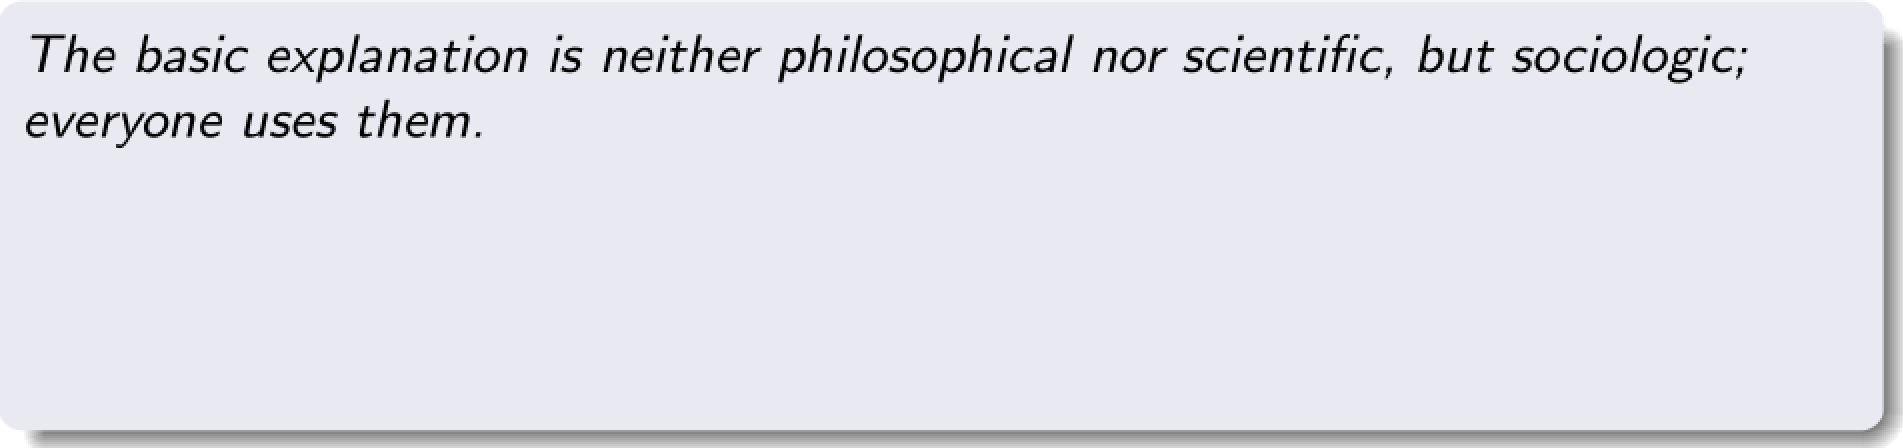
\includegraphics[width=11cm]{images/goodman_1}
    \end{center}
  \end{itemize}
  
\end{overlayarea}
\end{frame}
\begin{frame}
  \frametitle{Primer problema: interpretación del $p$-valor}
    \begin{overlayarea}{\textwidth}{0.8\textheight}
  ¿Qué solución podemos darle?\\ 
  Formación, conscienciación, pensamiento crítico?...\\
  Debemos ser conscientes (Goodman,
  2019, \href{https://doi.org/10.1080/00031305.2018.1558111}{The American Statistician} ):
  \begin{itemize}
  \item Los métodos científicos dentro de las disciplinas
    (oncología, física nuclear, genética, cardiología, producción
    animal, etc..) se enseñan y se transmiten dentro de estas mismas
    disciplinas. \onslide<+->{$\Rightarrow$ SILOS .}
  \item Es un problema sociológico. 
    \begin{center}
      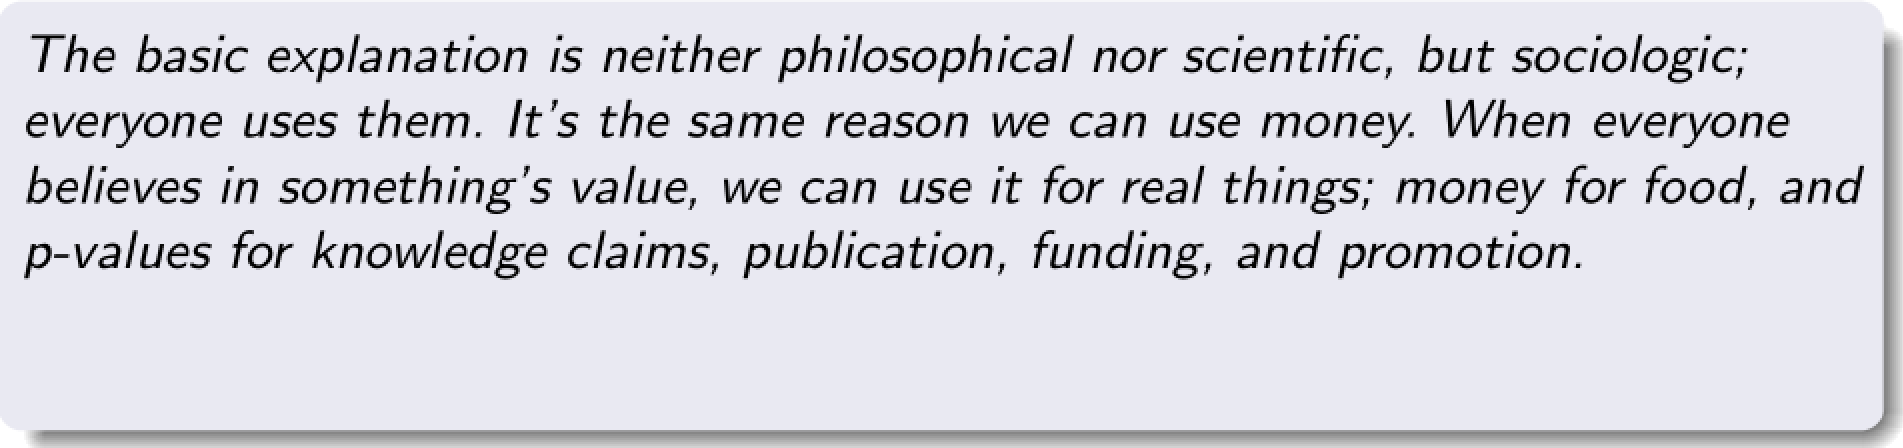
\includegraphics[width=11cm]{images/goodman_2}
    \end{center}
  \end{itemize}
  
\end{overlayarea}
\end{frame}
\begin{frame}
  \frametitle{Primer problema: interpretación del $p$-valor}
    \begin{overlayarea}{\textwidth}{0.8\textheight}
  ¿Qué solución podemos darle?\\
  Formación, conscienciación, pensamiento crítico?...\\
  Debemos ser conscientes (Goodman,
  2019, \href{https://doi.org/10.1080/00031305.2018.1558111}{The American Statistician} ):
  \begin{itemize}
  \item Los métodos científicos dentro de las disciplinas
    (oncología, física nuclear, genética, cardiología, producción
    animal, etc..) se enseñan y se transmiten dentro de estas mismas
    disciplinas. {$\Rightarrow$ SILOS .}
  \item Es un problema sociológico. 
    \begin{center}
      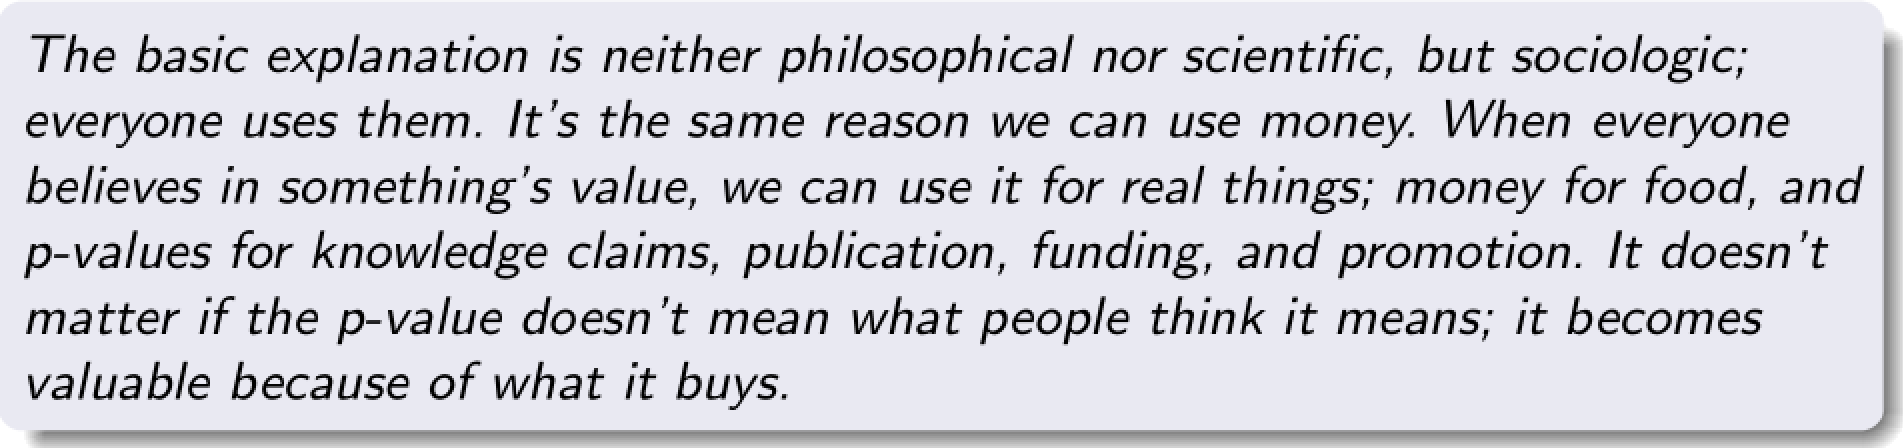
\includegraphics[width=11cm]{images/goodman_0}
    \end{center}      
  \item<2-> \textit{($\ldots$) the use of statistics tests has become
      obligatory in scientific research.($\ldots$)they work mainly as \textbf{social technologies}, not as guides to \textbf{private thinking}.
} 
  \end{itemize}
  
\end{overlayarea}
\end{frame}

\begin{frame}
  \frametitle{Primer problema: interpretación del $p$-valor}
    \begin{overlayarea}{\textwidth}{0.8\textheight}
  ¿Qué solución podemos darle?\\
  Formación, conscienciación, pensamiento crítico?...\\
  Debemos ser conscientes (Goodman,
  2019, \href{https://doi.org/10.1080/00031305.2018.1558111}{The
    American Statistician} ): \onslide<+->
  \begin{itemize}
  \item Es una respuesta a un problema de confianza.\onslide<+->
    \begin{block}{}
      \textit{The advances of statistics in medicine must be understood as responses to problems of trust, which have been most acute in the context of regulatory and disciplinary confrontations.}
    \end{block}
  \item<+-> No será fácil cambiarlo\onslide<+->
  \end{itemize}
  \begin{center}
      
\includegraphics[width=11cm]{images/goodman_bayes_1}
    \end{center}
\end{overlayarea} 
\end{frame}

\begin{frame}
  \frametitle{Primer problema: interpretación del $p$-valor}
    \begin{overlayarea}{\textwidth}{0.8\textheight}
  ¿Qué solución podemos darle?\\
  Formación, conscienciación, pensamiento crítico?...\\
  Debemos ser conscientes (Goodman,
  2019, \href{https://doi.org/10.1080/00031305.2018.1558111}{The
    American Statistician} ): 
  \begin{itemize}
  \item Es una respuesta a un problema de confianza.
    \begin{block}{}
      \textit{The advances of statistics in medicine must be understood as responses to problems of trust, which have been most acute in the context of regulatory and disciplinary confrontations.}
    \end{block}
  \item<+-> No será fácil cambiarlo
  \end{itemize}
  \begin{center}
      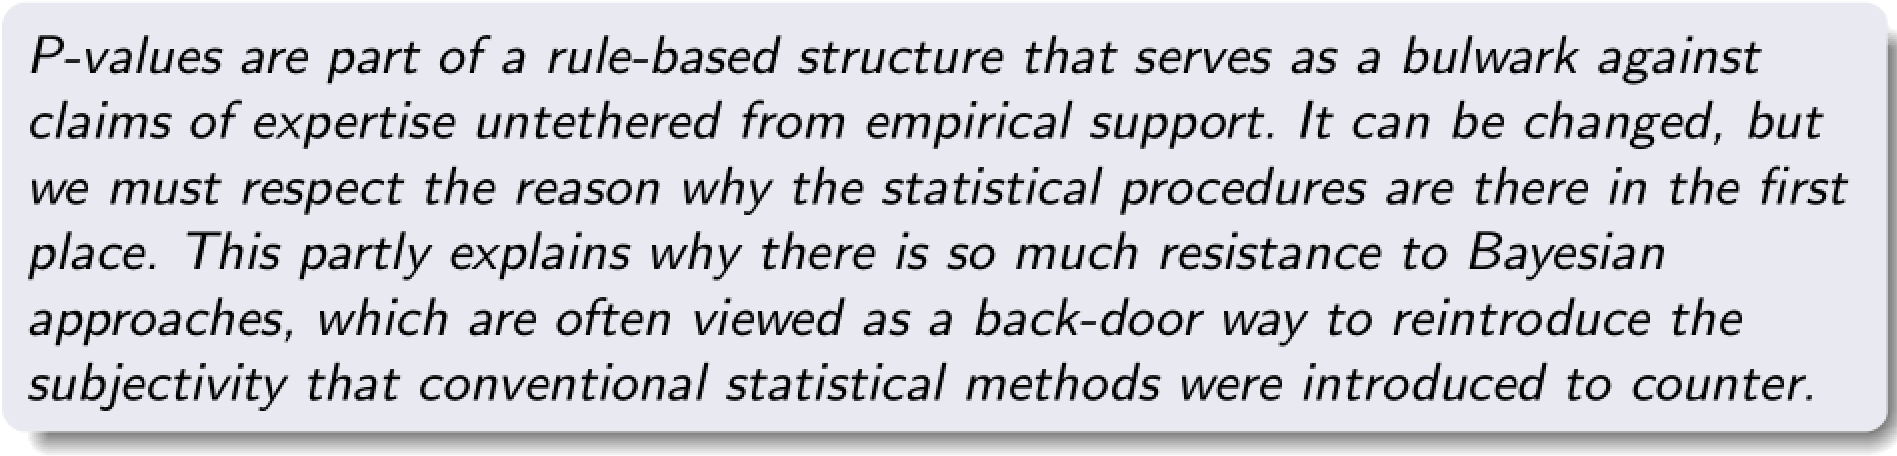
\includegraphics[width=11cm]{images/goodman_bayes_0}
    \end{center}
\end{overlayarea}
\end{frame}

\begin{frame}
  \frametitle{Primer problema: interpretación del $p$-valor}
  Una clara recomendación de
  \begin{itemize}
  \item   The American Statistical Association en Ronald L. Wasserstein, Allen L. Schirm \& Nicole A. Lazar (2019)
  Moving to a World Beyond ``$p < 0.05$'', \textit{The American
    Statistician}, 73:sup1,
  1-19. \href{https://doi.org/10.1080/00031305.2019.1583913}{enlace}

  \end{itemize}\medskip\onslide<2->

\begin{center}
  \Ovalbox{
    \begin{minipage}[h]{0.8\linewidth}
      \begin{center}
   \Huge No usemos nunca más el término ``Estadísticamente
   significativo''
         \end{center}
 \end{minipage}
   }\onslide<3->
 \end{center}\medskip
 
 Y ninguna de sus variantes: ``significativamente diferente'', ``$p < 0.05$'', ``no significativo'', en palabras o con estrellitas en una tabla.
\end{frame}

\begin{frame}
  \frametitle{Segundo problema: es el umbral $p = 0.05$ adecuado?}
    \begin{center}
      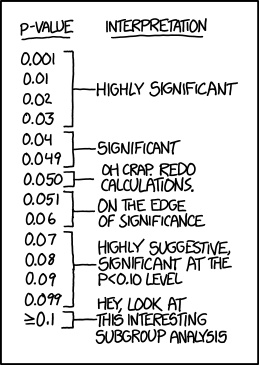
\includegraphics[height=0.8\textheight]{images/p_values_xkcd}
    \end{center}
    \hfill
    {\scriptsize \href{https://xkcd.com/1478/}{https://xkcd.com/1478/}}
  \end{frame}

  \begin{frame}
    \frametitle{Segundo problema: es el umbral $p = 0.05$ adecuado?}
    \begin{overlayarea}{\textwidth}{0.8\textheight}
    \begin{itemize}
    \item Desde inicio siglo XX, los científicos han ido adoptado un híbrido entre el enfoque de Fisher y
      el de Neyman \& Pearson (teoría
      decisión).\\ \onslide<2->{$\Leftrightarrow$ simplicidad del
        $p$-valor y (falsa) seguridad de la teoría de decisión, error,
        riesgo, etc...}\medskip
    \item<3-> Hay disciplinas en las que el umbral estándar es diferente:
      \begin{itemize}
      \item Genética: $p < 5\times 10^{-8}$ (para ``genome-wide
        association studies'')
      \item Física de altas energías: $ p < 3 \times 10^{-7}$ (``$3\sigma$'')
      \end{itemize}
    \end{itemize}\onslide<4->
    Es evidente que el valor del umbral debería tener en cuenta el
    contexto (tamaño muestral etc..)
  \end{overlayarea}
\end{frame}
\begin{frame}
    \frametitle{Segundo problema: es el umbral $p = 0.05$ adecuado?}
  
  \onslide<+->
    En \textit{Nature}, 567, 305-307, Marzo 2019:
    \begin{center}
      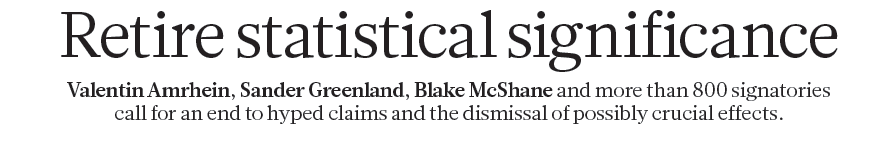
\includegraphics[width=7cm]{images/retire_statistical_significance}
    \end{center}
    \onslide<+->
    Dos estudios de análisis de efectos secundarios de medicamentos
    anti-inflamatorios:
    \begin{enumerate}
    \item El segundo equipo:\\ factor de riesgo de 1.2 (20\% más alto),
      IC: $[3\%, 48\%]$, ($p = 0.091$).\\
      \onslide<+-> $\Leftrightarrow$ ``La toma de estos medicamentos
      no está asociado con fibrilación auricular''. \onslide<+->
      \\ lo que contradice:
    \item<+-> El primer equipo:\\ factor de riesgo de 1.2 (20\% más alto),
      IC: $[9\%, 33\%]$, ($p = 0.0003$).\\
    \end{enumerate}
    \onslide<+->
      \begin{center}
      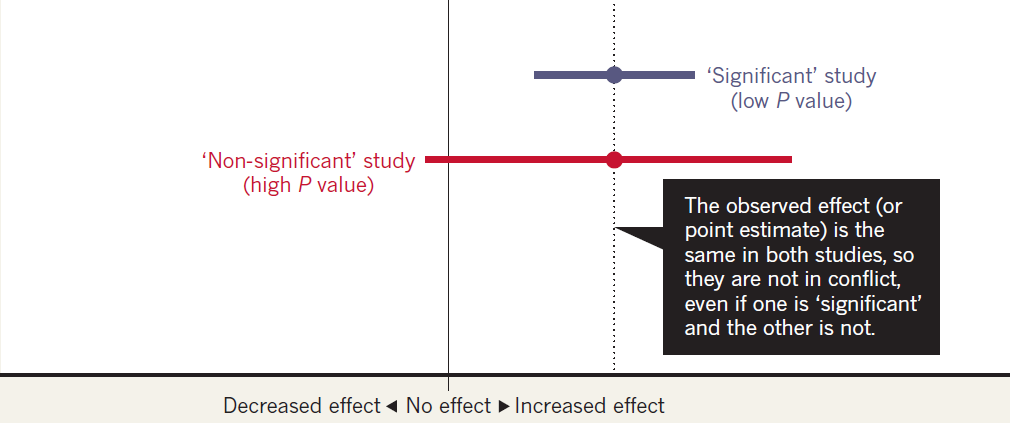
\includegraphics[width=6cm]{images/retire_statistical_significance_plot_cropped}
    \end{center}
  \end{frame}
  \begin{frame}
    \frametitle{Segundo problema: es el umbral $p = 0.05$ adecuado?}
    \begin{itemize}
    \item<+-> Es importante no limitarse a basar la decisión sobre
      significación científica sobre el único $p$-valor.
    \item<+-> $\Rightarrow$ hay que acompañarlo de estimación del
      efecto, con margen de error.
     \item<+-> $\Rightarrow$ hay que huir de la dicotomía basado en
       valor de $p$. 
     \end{itemize}\onslide<+->
     \begin{block}{}
       Es particularmente importante plantearse qué tamaño del efecto
       es relevante del punto de vista práctico.
     \end{block}\onslide<+->
     Es decir, hay que tener el contexto en cuenta.\onslide<+->
     \begin{itemize}
     \item      Rebecca A. Betensky (2019) The p-Value Requires Context, Not a Threshold, The American Statistician, 73:sup1, 115-117, \href{https://doi.org/10.1080/00031305.2018.1529624}{enlace}
     \end{itemize}
\onslide<+-> El contexto = tamaño relevante del efecto del punto de
vista práctico + tamaño muestral (diseño del experimento).
\end{frame}
  \begin{frame}
    \frametitle{Segundo problema: es el umbral $p = 0.05$ adecuado?}
    Esto tampoco es nuevo...\onslide<2->
    \begin{center}
\multiinclude[format=png,start=1]{images/gosset} %     \includegraphics[0.8\textheight]{images/gosset.png}
    \end{center}
\end{frame}
\begin{frame}
  \frametitle{Segundo problema: es el umbral $p = 0.05$ adecuado?}
  Ha habido varios propuestas para  calibrar el $p$-valor.\onslide<2->\\
  Varios introducen elementos Bayesianos.\\
  En particular las probabilidades a priori de las hipótesis y el
  factor Bayes: \onslide<3->
  $$\frac{\P\left({H}_{1}\left|{x}_{{\rm{obs}}}\right.\right)}{\P\left({H}_{0}\left|{x}_{{\rm{obs}}}\right.\right)}=\frac{f\left({x}_{{\rm{obs}}}\left|{H}_{1}\right.\right)}{f\left({x}_{{\rm{obs}}}\left|{H}_{0}\right.\right)}\times \frac{\P\left({H}_{1}\right)}{\P\left({H}_{0}\right)}\equiv {\rm{BF}}\times \left({\rm{prior}}\,{\rm{odds}}\right)
  $$\onslide<4->
  Aquí aparece $\P\left({H}_{0}\left|{x}_{{\rm{obs}}}\right.\right)$,
  que es el FPR (False Positive Risk).\onslide<5->\\
  {\scriptsize T. Sellke; M. J. Bayarri; J. O. Berger (2001), ``Calibration of p Values for Testing Precise Null Hypotheses'', \textit{
The American Statistician}, 55:1, pp. 62-71.}\onslide<6->
  \begin{block}{Simulación sencilla}
    \begin{itemize}
    \item<7-> Contexto: ensayos medicamentos. $D_1,D_2, \ldots D_N$
      situaciones similares de medicamentos y sus ensayos.
    \item<8-> Se asume $\P(H_0) = 0.5$. Se simula para cada $D_i$ la
      hipótesis, habiendo escogido el tamaño relevante del efecto si $H_1$
    \item<9-> Se simulan ensayos independientes para cada $D_i$ 
    \end{itemize}
    \onslide<10-> Entre los $D_i$ para los cuales $p\simeq 0.05$, como
    mínimo el 23\% no presenta efecto, es decir $H_0$ cierta.
  \end{block}
\end{frame}
\begin{frame}
  \frametitle{Segundo problema: es el umbral $p = 0.05$ adecuado?}
      \begin{overlayarea}{\textwidth}{\textheight}
    Recientemente (2017), en Nature Human Behaviour, 70 autores:\\
      \begin{center}
\multiinclude[format=png,start=1]{images/redefine} %     \includegraphics[0.8\textheight]{images/gosset.png}
    \end{center}
  \end{overlayarea}
\end{frame}
\begin{frame}
  \frametitle{Segundo problema: es el umbral $p = 0.05$ adecuado?}
      \begin{overlayarea}{\textwidth}{\textheight}
  Recientemente (2017), en Nature Human Behaviour, 70 autores:\\
     Para justificarlo, consideran factor Bayes: \onslide<2->
   $$\frac{\P\left({H}_{1}\left|{x}_{{\rm{obs}}}\right.\right)}{\P\left({H}_{0}\left|{x}_{{\rm{obs}}}\right.\right)}=\frac{f\left({x}_{{\rm{obs}}}\left|{H}_{1}\right.\right)}{f\left({x}_{{\rm{obs}}}\left|{H}_{0}\right.\right)}\times \frac{\P\left({H}_{1}\right)}{\P\left({H}_{0}\right)}\equiv {\rm{BF}}\times \left({\rm{prior}}\,{\rm{odds}}\right)
  $$\onslide<3->
  En un caso sencillo, usando cuotas para el BF:\onslide<4->
  \begin{center}
    \includegraphics[width=7.5cm]{images/redefine_plot}
  \end{center}\vspace{-0.5cm}\onslide<5->
  \begin{block}{}
    \begin{itemize}
    \item Para $p \simeq 0.05$, $2.5\leq BF\leq 3.4$ ``weak o very
      weak evidence''
    \item Para $p \simeq 0.005$, $14\leq BF\leq 26$ ``sustancial or strong''
    \end{itemize}
  \end{block}
  
  \end{overlayarea}
\end{frame}
\begin{frame}
  \frametitle{Tercer problema: $p$-hacking}
  ¿Qué es el $p$-hacking?\onslide<2->
  \begin{block}{$p$-hacking, popularizado por Uri Simonsohn, psicólogo
      U. Pensilvania}
    ``$p$-hacking is trying multiple things until you get the desired result''
  \end{block}
  \onslide<3->
  \begin{center}
    \includegraphics[width=5cm]{images/torture}
  \end{center}
  \hfill
    {\scriptsize \href{https://statistically-funny.blogspot.com/2014/}{https://statistically-funny.blogspot.com/2014/}}
\end{frame}
\begin{frame}
  \frametitle{Tercer problema: $p$-hacking}
  Muy recomendable: Seminario, julio 2018 ``Reliable Research in
  Business'', University of Florida, Warrington College of Business \href{https://youtu.be/8wDwcp1EwNM}{youtube}
  \begin{center}
    \includegraphics[width=9cm]{images/p-hacking}
  \end{center}
\end{frame}
\begin{frame}
  \frametitle{Tercer problema: $p$-hacking}

  \begin{itemize}
  \item<2-> El $p$-hacking no se realiza con intención de fraude. 
  \item<3-> Puede ser incluso inconsciente, una tentación natural
  \item<4-> Nace de la presión por publicar. 
  \end{itemize}\onslide<5->
  \begin{block}{}
    Puede tomar la forma de varios mecanismos, que se pueden resumir todos
  como ``selective reporting''.
\end{block}\onslide<6->
Mencionamos dos de ellos:
\begin{enumerate}
\item File drawering
\item Cherry picking 
\end{enumerate}
\end{frame}
\begin{frame}
  \frametitle{Tercer problema: $p$-hacking}
  \begin{block}{File drawering}
    Consiste en meter en el cajón los experimentos cuyos resultados
    salen no significativos.
  \end{block}\onslide<2->
  ¿Por qué? \onslide<3->{Por la presión de publicar.}\\ \onslide<4-> Recordad: Ioannidis (2019), Entre los
  abstracts que contienen un $p$-valor el 96\% tienen
  $p<0.05$.\\
  \onslide<5-> Sin embargo, no parece común, por el coste que supone.
  
\end{frame}
\begin{frame}
  \frametitle{Tercer problema: $p$-hacking}
  \begin{block}{Cherry picking}
    Escoger las cerezas en la tarta, o en la cesta... Escoger sólo los
    mejores resultados
  \end{block}\onslide<2->
  Se puede hacer de varias maneras.
  \begin{itemize}
  \item<3-> Sólo escogiendo variables que presentan efecto significativo.
  \item<4-> Sólo me quedo con algunas covariables.
  \item<5-> Adaptando el tamaño de la muestra: si no tengo resultados
    significativos, sigo recogiendo datos.
  \item<6-> y más...
  \end{itemize}\onslide<7->
  \begin{block}{}
    Es muy fácil comprobar el efecto del ``cherry-picking'' por
    simulaciones, y tiene un gran valor pedagógico.
  \end{block}
\end{frame}

\begin{frame}
  \frametitle{Tercer problema: $p$-hacking.}
  Para simular la elección selectiva de variables:\\ \onslide<2->
  \begin{block}{Planteamiento}
    \begin{itemize}
    \item     En mi experimento, considero dos variables $X$ e $Y$,
      posiblemente correladas.
    \item Quiero probar si presentan efecto, es decir $\mu_X \neq 0$,
      $\mu_Y\neq 0$.
    \item   Publico siempre, sea cual sea el resultado del
      experimento, pero
      \begin{itemize}
      \item si solo uno de los dos $p$-valores, $p_x$ o $p_y$ es menor
        de 0.05, sólo publico el resultado sobre esa variable.
      \end{itemize}
    \end{itemize}

  \end{block}\onslide<3->
  \begin{center}
%     \begin{tabular}[h]{lllll}
%       Muestra&$Z_X$&$Z_Y$&$p_X$&$p_Y$\\
%       1 & -0.918 & 0.167 & 0.359 & 0.867 \\
% 2 & -1.12 & 0.178 & 0.261 & 0.858 \\
% 3 & -0.327 & -1.50 & 0.744 & 0.134 \\
% 4 & -1.70 & -1.63 & 0.0899 & 0.103 \\
%       5 & -0.246 & 0.457 & 0.806 & 0.648 \\
%       \vdots&\vdots&\vdots&\vdots&\vdots\\
%       59 & -0.345 & 1.99 & 0.730 & 0.0462\\
%       \vdots&\vdots&\vdots&\vdots&\vdots\\
%       170 & 2.54 & 2.20 & 0.0110 & 0.0276\\
%       \vdots&\vdots&\vdots&\vdots&\vdots
                                     %       \end{tabular}
    \includegraphics[width=0.5\linewidth]{images/select_variable-1}
  \end{center}
\end{frame}
\begin{frame}
  \frametitle{Tercer problema: $p$-hacking.}
  Para simular la elección selectiva de variables:\\ 
  \begin{block}{Planteamiento}
    \begin{itemize}
    \item     En mi experimento, considero dos variables $X$ e $Y$,
      posiblemente correladas.
    \item Quiero probar si presentan efecto, es decir $\mu_X \neq 0$,
      $\mu_Y\neq 0$.
    \item   Publico siempre, sea cual sea el resultado del
      experimento, pero
      \begin{itemize}
      \item si solo uno de los dos $p$-valores, $p_x$ o $p_y$ es menor
        de 0.05, sólo publico el resultado sobre esa variable.
      \end{itemize}
    \end{itemize}

  \end{block}
  \begin{center}
    \includegraphics[width=0.5\linewidth]{images/select_variable-2}
  \end{center}
\end{frame}

\begin{frame}
  \frametitle{Tercer problema: $p$-hacking.}
  Para simular la elección selectiva de variables:\\ 
  \begin{block}{Planteamiento}
    \begin{itemize}
    \item     En mi experimento, considero dos variables $X$ e $Y$,
      posiblemente correladas.
    \item Quiero probar si presentan efecto, es decir $\mu_X \neq 0$,
      $\mu_Y\neq 0$.
    \item   Publico siempre, sea cual sea el resultado del
      experimento, pero
      \begin{itemize}
      \item si solo uno de los dos $p$-valores, $p_x$ o $p_y$ es menor
        de 0.05, sólo publico el resultado sobre esa variable.
      \end{itemize}
    \end{itemize}

  \end{block}
  \begin{center}
    \includegraphics[width=0.5\linewidth]{images/select_variable-3} 
  \end{center}
\end{frame}

\begin{frame}
  \frametitle{Tercer problema: $p$-hacking.}
  Para simular la elección selectiva de variables:\\
  \begin{center}
    \includegraphics[height=0.9\textheight]{images/R-script-1}
  \end{center}
\end{frame}

% \begin{frame}
%   \frametitle{Tercer problema: $p$-hacking.}
%   \begin{overlayarea}{\textwidth}{\textheight}
%   Para simular la elección selectiva de variables:\alert{(con
%     {\tt purrr})}.\\
%   \hspace*{-1cm}
%   \includegraphics[width=1.2\textwidth]{images/R-script-1_sinoptico}
% \end{overlayarea}
% \end{frame}

\begin{frame}
  \frametitle{Tercer problema: $p$-hacking.}
  \begin{overlayarea}{\textwidth}{\textheight}
  Para simular la elección selectiva de variables:\\
  \begin{center}
  \includegraphics[width=7cm]{images/resultados_seleccion_variable}    
  \end{center}

\end{overlayarea}
\end{frame}

\begin{frame}
  \frametitle{Tercer problema: $p$-hacking.}
  Para simular la parada selectiva de recogida de datos:\\ \onslide<2->
  \begin{block}{Planteamiento}
    \begin{itemize}
    \item     En mi experimento, considero un variable $X$ 
    \item Quiero probar si presenta efecto, es decir $\mu_X \neq 0$.
    \item   Publico siempre, sea cual sea el resultado del
      experimento, pero
      \begin{itemize}
      \item Empiezo por coger una muestra de 20. Si  $p_x \geq 0.05$,
        cojo otros 10 y vuelvo a calcular $p$-valor.
      \end{itemize}
    \end{itemize}

  \end{block}\onslide<3->
  \begin{center}
%     \begin{tabular}[h]{lllll}
%       Muestra&$Z_X$&$p_X$&$Z_X^{hacked}$&$p_X^{hacked}$\\
% 1 & 0.185 & 0.853 & -0.450 & 0.653\\
% 2 & 1.31 & 0.190 & 1.00 & 0.316\\
% 3 & 0.493 & 0.622 & 1.20 & 0.230\\
% 4 & -0.842 & 0.400 & -0.421 & 0.673\\
% 5 & 1.37 & 0.170 & 1.33 & 0.182\\
%       \vdots&\vdots&\vdots&\vdots&\vdots\\
%         26 & -2.30 & 0.0214 & -2.30 & 0.0214\\
%       \vdots&\vdots&\vdots&\vdots&\vdots\\
%   43 & -1.29 & 0.197 & -2.18 & 0.0291\\
%       \vdots&\vdots&\vdots&\vdots&\vdots
%                                            \end{tabular}

    \includegraphics[width=0.5\linewidth]{images/select_size-1} 
  \end{center}
\end{frame}

\begin{frame}
  \frametitle{Tercer problema: $p$-hacking.}
  Para simular la parada selectiva de recogida de datos:\\ 
  \begin{block}{Planteamiento}
    \begin{itemize}
    \item     En mi experimento, considero un variable $X$ 
    \item Quiero probar si presenta efecto, es decir $\mu_X \neq 0$.
    \item   Publico siempre, sea cual sea el resultado del
      experimento, pero
      \begin{itemize}
      \item Empiezo por coger una muestra de 20. Si  $p_x \geq 0.05$,
        cojo otros 10 y vuelvo a calcular $p$-valor.
      \end{itemize}
    \end{itemize}

  \end{block}
  \begin{center}
    \includegraphics[width=0.5\linewidth]{images/select_size-2} 
  \end{center}
\end{frame}
\begin{frame}
  \frametitle{Tercer problema: $p$-hacking.}
  Para simular la parada selectiva de recogida de datos:\\ 
  \begin{block}{Planteamiento}
    \begin{itemize}
    \item     En mi experimento, considero un variable $X$ 
    \item Quiero probar si presenta efecto, es decir $\mu_X \neq 0$.
    \item   Publico siempre, sea cual sea el resultado del
      experimento, pero
      \begin{itemize}
      \item Empiezo por coger una muestra de 20. Si  $p_x \geq 0.05$,
        cojo otros 10 y vuelvo a calcular $p$-valor.
      \end{itemize}
    \end{itemize}

  \end{block}
  \begin{center}
    \includegraphics[width=0.5\linewidth]{images/select_size-3} 
  \end{center}
\end{frame}

\begin{frame}
  \frametitle{Tercer problema: $p$-hacking.}
  \begin{overlayarea}{\textwidth}{\textheight}
  Para simular la parada selectiva de recogida de datos:
  \begin{center}
    \includegraphics[height=0.9\textheight]{images/R-script-2}
  \end{center}
\end{overlayarea}
\end{frame}

% \begin{frame}
%   \frametitle{Tercer problema: $p$-hacking.}
%     \begin{overlayarea}{\textwidth}{\textheight}
%   Para simular la parada selectiva de recogida de datos: \alert{(con
%   {\tt purrr})}.\\
% \hspace*{-0.8cm}\includegraphics[width=1.2\textwidth]{images/R-script-2_purrr}
% \end{overlayarea}
% \end{frame}

\begin{frame}
  \frametitle{Tercer problema: $p$-hacking.}
    \begin{overlayarea}{\textwidth}{\textheight}
  Para simular la parada selectiva de recogida de datos: \\
\begin{center}
\includegraphics[width=7cm]{images/resultados_select_size}  
\end{center}

\end{overlayarea}
\end{frame}

\begin{frame}
  \frametitle{Tercer problema: $p$-hacking.}
    \begin{overlayarea}{\textwidth}{\textheight}
      Ejemplo en A/B testing: \\
      \onslide<+->
      \begin{block}{Qué es el A/B testing? \href{https://www.abtasty.com/es/ab-testing/}{Extraido de https://www.abtasty.com/es/ab-testing/}}
El A/B testing consiste en comparar dos versiones de una misma página web o aplicación para comprobar cuál de las dos versiones es más eficiente. Estas variaciones, llamadas A y B, se muestran de forma aleatoria a los distintos usuarios de la página web. Una parte de ellos verá la versión A y la parte restante verá la versión B.
      \end{block}
\end{overlayarea}
\end{frame}

\begin{frame}
  \frametitle{Tercer problema: $p$-hacking.}
    \begin{overlayarea}{\textwidth}{\textheight}
      \begin{center}
\includegraphics[width=10cm]{images/ab_testing}  
\end{center}
\end{overlayarea}
\end{frame}

\begin{frame}
  \frametitle{Tercer problema: $p$-hacking.}
  ¿Qué solución para el $p$-hacking?\onslide<+->
  \begin{itemize}
  \item<+-> Concienciación.
  \item<+-> Pedir que se publiquen todos los experimentos realizados
  \item<+-> Distinguir muy bien entre experimento exploratorio y
    experimento para investigar efecto.   
  \end{itemize}
  \onslide<+-> Esto se puede abordar pidiendo el pre-registro de los
  experimentos antes de la publicación.\\ 
  \onslide<+-> Por ejemplo, en
  \href{https://aspredicted.org}{aspredicted.org}\\
  \onslide<+-> Eso es parte de Open science.
  
\end{frame}

\begin{frame}
  \frametitle{Tercer problema: $p$-hacking.}
  \hspace*{-0.5cm}\includegraphics[height=1.0\textheight]{images/aspredicted_web-0}
\end{frame}
\begin{frame}
  \frametitle{Tercer problema: $p$-hacking.}
    \hspace*{-0.5cm}\includegraphics[height=1.0\textheight]{images/aspredicted_web-1}
\end{frame}

\begin{frame}
  \frametitle{Tercer problema: $p$-hacking.}
    \hspace*{-0.5cm}\includegraphics[height=1.0\textheight]{images/aspredicted_web-2}
\end{frame}
\begin{frame}
  \frametitle{Tercer problema: $p$-hacking.}
    \hspace*{-0.5cm}\includegraphics[height=1.0\textheight]{images/aspredicted_web-3}
\end{frame}
\begin{frame}
  \frametitle{Tercer problema: $p$-hacking.}
    \hspace*{-0.5cm}\includegraphics[height=0.9\textheight]{images/aspredicted_sample}
\end{frame}

\begin{frame}
  \frametitle{Conclusiones}
  Merece la pena recorrer las recomendaciones de
  
  \begin{block}{}
  R. Wasserstein, A. Schirm \& N. Lazar (2019)
  Moving to a World Beyond ``$p < 0.05$'', \textit{The American
    Statistician}, 73:sup1,
  1-19. \href{https://doi.org/10.1080/00031305.2019.1583913}{enlace}
    
\end{block}\onslide<2->
Las resumen en:\medskip
\begin{center}
  \Ovalbox{\Huge ATOM}
\end{center}

\onslide<3->
\begin{block}{}
  \begin{itemize}
  \item \textbf{\Huge A}ccept uncertainty.
  \item Be \textbf{\Huge T}houghtful.
   \item Be \textbf{\Huge O}pen.
   \item Be \textbf{\Huge M}odest. 
  \end{itemize}
\end{block}

\end{frame}

\begin{frame}
  \frametitle{Conclusiones: ATOM}
\onslide<2->
  \begin{block}{}
  \begin{itemize}
  \item \textbf{\Huge A}ccept uncertainty.
  \end{itemize}
\end{block}

\begin{itemize}
\item<3-> Los métodos estadísticos no quitan la incertidumbre presente en
  los datos.
\item<4-> Presenta estimaciones de los efectos con su margen de error.
\item<5-> Es bueno realizar estudios de réplica, hay que aceptar que
  pueden proporcionar resultados diferentes.
\end{itemize}
\onslide<6->
\begin{block}{}
  \begin{itemize}
  \item Be \textbf{\Huge T}houghtful.
  \end{itemize}
\end{block}


\begin{itemize}
\item<7-> Es recomendable reflexionar sobre muchos aspectos:
  \begin{itemize}
  \item Cuáles son las consecuencias prácticas del estimador?.  Cuál es
    su precisión? El modelo está bien especificado?
  \end{itemize}
 
\item<8-> Ten en cuenta el contexto científico y el conocimiento
  previo:
  \begin{itemize}
  \item Qué magnitud del efecto es relevante en la práctica? Eso antes
    de recoger datos.
  \end{itemize}
\item<9-> Considera más que sólo el $p$-valor en la decisión:
  aspectos prácticos, calidad de los datos, conocimiento previo,
  etc...
\item<10-> Complementa $p$-valor con otras medidas, considerar otras metodologías. 
\end{itemize}

\end{frame}

\begin{frame}
  \frametitle{Conclusiones: ATOM}

  \begin{block}{}
  \begin{itemize}
  \item Be \textbf{\Huge O}pen.
  \end{itemize}
\end{block}

\begin{itemize}
\item<2-> Abierto a la transparencia, abierto a las prácticas de
  ``Open Science'' (preregistro, comparte datos, comparte código, etc...)
\item<3-> Abierto en la comunicación de los resultados.
\item<4-> Abierto al hecho de que, a menudo, un estudio no es suficiente. 
\end{itemize}
\onslide<5->
\begin{block}{}
  \begin{itemize}
  \item Be \textbf{\Huge M}odest
  \end{itemize}
  
\end{block}
\begin{itemize}
\item<6-> No confundas estadística y realidad. Un modelo siempre es
  una representación extremadamente simplificada de la
  realidad. $\Rightarrow$ hay muchos modelos posibles.
\item<7-> Sé consciente de las limitaciones de los métodos estadísticos.
\item<8-> Anima otros a replicar tu trabajo.

\item<9-> Acepta que siempre habrá incertidumbre.
\end{itemize}

\end{frame}


\begin{frame}
  \frametitle{Recursos utilizados}
  \begin{itemize}
  \item Mathieu Kessler, Elías Moreno (2015) It is forbidden to use p-values!  BEIO, 31:2, 1 June 2015, 202-206
\href{http://www.seio.es/BBEIO/BEIOVol31Num2}{http://www.seio.es/BBEIO/BEIOVol31Num2}

\item David Trafimow \& Michael Marks (2015) Editorial, Basic and Applied Social Psychology, 37:1, 1-2 \href{http://dx.doi.org/10.1080/01973533.2015.1012991}{http://dx.doi.org/10.1080/01973533.2015.1012991}

\item Nuzzo (2014) "Scientific method: statistical errors", Nature, News feature. \href{https://www.nature.com/news/scientific-method-statistical-errors-1.14700}{https://www.nature.com/news/scientific-method-statistical-errors-1.14700}

  \item Ronald L. Wasserstein \& Nicole A. Lazar (2016) The ASA's Statement on p-Values: Context, Process, and Purpose, The American Statistician, 70:2, 129-133,  \href{https://doi.org/10.1080/00031305.2016.1154108}{https://doi.org/10.1080/00031305.2016.1154108}

  \item ASA symposium on statistical Inference: october 11-13, 2017
    "Scientific methods for the 21st century: A World Beyond $p < 0.05$.\\ 
\textbf{Grabación de las sesiones:}
\href{http://ww2.amstat.org/meetings/ssi/2017/recordedsessions.cfm}{enlace}

\item Special issue The American Statistician:  Vol 73, March 2019, Issue 1.
Statistical Inference in the 21st Century: A World Beyond $p < 0.05$. \href{https://www.tandfonline.com/toc/utas20/73/sup1}{enlace}
\end{itemize}
\end{frame}

\begin{frame}
  \frametitle{Recursos utilizados}
  \begin{itemize}

\item Podcast Roger Peng y Hilary Parker. "Not so standard deviations", \href{http://nssdeviations.com/}{http://nssdeviations.com/}. Episode 77, "Back to statistics".

\item The reproducibility crisis in science: A statistical counterattack, Roger Peng, 
First published: 15 June 2015 \href{https://doi.org/10.1111/j.1740-9713.2015.00827.x}{enlace}

\item La depresión del Excel, Paul Krugman El pais 21 abril 2013 \href{https://elpais.com/economia/2013/04/19/actualidad/1366398440_370422.html}{enlace}

\item Estimating the reproducibility of psychological science Open Science Collaboration*,†
(270 autores), Science 28 Aug 2015, Vol. 349, Issue 6251 \href{http://science.sciencemag.org/content/349/6251/aac4716}{enlace}

\item Nature "Challenges in irreproducible research", 2018. \href{https://www.nature.com/collections/prbfkwmwvz}{https://www.nature.com/collections/prbfkwmwvz}

  \item Final report - Science as an open enterprise, The Royal Society, 2012 \href{https://royalsociety.org/topics-policy/projects/science-public-enterprise/report/}{enlace}

  \item El portal de la Unión Europea sobre Open Science \href{https://ec.europa.eu/research/openscience/index.cfm}{enlace}

  \item John P. A. Ioannidis (2019) What Have We (Not) Learnt from
    Millions of Scientific Papers with P Values?, The American
    Statistician, 73:sup1, 20-25, \href{https://doi.org/10.1080/00031305.2018.1447512}{enlace}

  \item Steven N. Goodman (2019) Why is Getting Rid of P-Values So Hard? Musings on Science and Statistics, The American Statistician, 73:sup1, 26-30, \href{https://doi.org/10.1080/00031305.2018.1558111}{enlace}

  \end{itemize}
\end{frame}

\begin{frame}
  \frametitle{Recursos utilizados}
  \begin{itemize}

\item Valentin Amrheim, Sander Greenland, Blake McShane (2019) "Retire
  Statistical Significance", Nature, 567, 305-307, \href{https://www.nature.com/articles/d41586-019-00857-9}{enlace}

  
\item Thomas Sellke, M. J Bayarri \& James O Berger (2001) Calibration
  of $p$-Values for Testing Precise Null Hypotheses, The American Statistician, 55:1, 62-71, \href{https://doi.org/10.1198/000313001300339950}{enlace}

  
\item Benjamin, D. J., Berger, J. O., Johannesson, M., Nosek, B. A.,
  Wagenmakers, E. J., Berk, R., Bollen, K. A., Brembs, B., Brown, L.,
  Camerer, C., and Cesarini, D. (2018), “Redefine Statistical
  Significance,” Nature Human Behaviour, 2, 6. [115,117]
  \href{https://www.nature.com/articles/s41562-017-0189-z}{enlace}

\item Charla ``Life after $p$-hacking'', John Simons en el seminario de julio 2018 ``Reliable Research in
  Business'', University of Florida, Warrington College of Business
  \href{https://youtu.be/8wDwcp1EwNM}{youtube} 
\item Recomiendo explorar para R los paquetes y la filosofia del
  ``Tidyverse'', promovido por RStudio y
  colaboradores. Particularmente interesante es la librería ``dplyr''
  y ``purrr''. \href{https://www.tidyverse.org/}{https://www.tidyverse.org/}
\end{itemize}
\end{frame}
\end{document}
